% Options for packages loaded elsewhere
\PassOptionsToPackage{unicode}{hyperref}
\PassOptionsToPackage{hyphens}{url}
\PassOptionsToPackage{dvipsnames,svgnames,x11names}{xcolor}
%
\documentclass[11pt,a4paper]{article}
\usepackage[scale=0.8]{geometry}
\usepackage{rotating}
\usepackage{amsmath,amssymb}
\usepackage{iftex}
\ifPDFTeX
  \usepackage[T1]{fontenc}
  \usepackage[utf8]{inputenc}
  \usepackage{textcomp} % provide euro and other symbols
\else % if luatex or xetex
  \usepackage{unicode-math}
  \defaultfontfeatures{Scale=MatchLowercase}
  \defaultfontfeatures[\rmfamily]{Ligatures=TeX,Scale=1}
\fi
\usepackage{lmodern}
\ifPDFTeX\else  
    % xetex/luatex font selection
\fi
% Use upquote if available, for straight quotes in verbatim environments
\IfFileExists{upquote.sty}{\usepackage{upquote}}{}
\IfFileExists{microtype.sty}{% use microtype if available
  \usepackage[]{microtype}
  \UseMicrotypeSet[protrusion]{basicmath} % disable protrusion for tt fonts
}{}

\usepackage{xcolor}
\setlength{\emergencystretch}{3em} % prevent overfull lines
\setcounter{secnumdepth}{5}
% Make \paragraph and \subparagraph free-standing
\makeatletter
\ifx\paragraph\undefined\else
  \let\oldparagraph\paragraph
  \renewcommand{\paragraph}{
    \@ifstar
      \xxxParagraphStar
      \xxxParagraphNoStar
  }
  \newcommand{\xxxParagraphStar}[1]{\oldparagraph*{#1}\mbox{}}
  \newcommand{\xxxParagraphNoStar}[1]{\oldparagraph{#1}\mbox{}}
\fi
\ifx\subparagraph\undefined\else
  \let\oldsubparagraph\subparagraph
  \renewcommand{\subparagraph}{
    \@ifstar
      \xxxSubParagraphStar
      \xxxSubParagraphNoStar
  }
  \newcommand{\xxxSubParagraphStar}[1]{\oldsubparagraph*{#1}\mbox{}}
  \newcommand{\xxxSubParagraphNoStar}[1]{\oldsubparagraph{#1}\mbox{}}
\fi
\makeatother


\providecommand{\tightlist}{%
  \setlength{\itemsep}{0pt}\setlength{\parskip}{0pt}}\usepackage{longtable,booktabs,array}
\usepackage{calc} % for calculating minipage widths
% Correct order of tables after \paragraph or \subparagraph
\usepackage{etoolbox}
\makeatletter
\patchcmd\longtable{\par}{\if@noskipsec\mbox{}\fi\par}{}{}
\makeatother
% Allow footnotes in longtable head/foot
\IfFileExists{footnotehyper.sty}{\usepackage{footnotehyper}}{\usepackage{footnote}}
\makesavenoteenv{longtable}
\usepackage{graphicx}
\makeatletter
\def\maxwidth{\ifdim\Gin@nat@width>\linewidth\linewidth\else\Gin@nat@width\fi}
\def\maxheight{\ifdim\Gin@nat@height>\textheight\textheight\else\Gin@nat@height\fi}
\makeatother
% Scale images if necessary, so that they will not overflow the page
% margins by default, and it is still possible to overwrite the defaults
% using explicit options in \includegraphics[width, height, ...]{}
\setkeys{Gin}{width=\maxwidth,height=\maxheight,keepaspectratio}
% Set default figure placement to htbp
\makeatletter
\def\fps@figure{htbp}
\makeatother

% \addtolength{\oddsidemargin}{-.5in} % superseded by the official template dimensions%
% \addtolength{\evensidemargin}{-.1in} % superseded by the official template dimensions%
% \addtolength{\textwidth}{1in} % superseded by the official template dimensions%
% \addtolength{\textheight}{1.7in} % superseded by the official template dimensions%
% \addtolength{\topmargin}{-1in} % superseded by the official template dimensions
\makeatletter
\@ifpackageloaded{caption}{}{\usepackage{caption}}
\AtBeginDocument{%
\ifdefined\contentsname
  \renewcommand*\contentsname{Table of contents}
\else
  \newcommand\contentsname{Table of contents}
\fi
\ifdefined\listfigurename
  \renewcommand*\listfigurename{List of Figures}
\else
  \newcommand\listfigurename{List of Figures}
\fi
\ifdefined\listtablename
  \renewcommand*\listtablename{List of Tables}
\else
  \newcommand\listtablename{List of Tables}
\fi
\ifdefined\figurename
  \renewcommand*\figurename{Figure}
\else
  \newcommand\figurename{Figure}
\fi
\ifdefined\tablename
  \renewcommand*\tablename{Table}
\else
  \newcommand\tablename{Table}
\fi
}
\@ifpackageloaded{float}{}{\usepackage{float}}
\floatstyle{ruled}
\@ifundefined{c@chapter}{\newfloat{codelisting}{h}{lop}}{\newfloat{codelisting}{h}{lop}[chapter]}
\floatname{codelisting}{Listing}
\newcommand*\listoflistings{\listof{codelisting}{List of Listings}}
\makeatother
\makeatletter
\makeatother
\makeatletter
\@ifpackageloaded{caption}{}{\usepackage{caption}}
\@ifpackageloaded{subcaption}{}{\usepackage{subcaption}}
\makeatother


\ifLuaTeX
  \usepackage{selnolig}  % disable illegal ligatures
\fi
\usepackage[round,sectionbib]{natbib}
\setlength{\bibsep}{0pt plus 0.3ex}
%\usepackage{doi}
\bibliographystyle{abbrvnat}
\usepackage{bookmark}

\IfFileExists{xurl.sty}{\usepackage{xurl}}{} % add URL line breaks if available
\urlstyle{same} % disable monospaced font for URLs
\usepackage{mathabx}
\usepackage{authblk}
\usepackage{enumerate}
\usepackage{threeparttable}
\usepackage{pdflscape}
\usepackage{newtxtext}
\newtheorem{definition}{Definition}
\newtheorem{corollary}{Corollary}
\newtheorem{lemma}{Lemma}
\newtheorem{theorem}{Theorem}
\newtheorem{assumption}{Assumption}
\newtheorem{remark}{Remark}
\newtheorem{passumption}{Assumption}
\renewcommand{\thepassumption}{\arabic{passumption}$'$}

\usepackage{siunitx}
\sisetup{detect-all}
\newcolumntype{d}[1]{S[table-format=#1]}


\title{Quasi-Maximum Likelihood Estimation for a Genuinely Unbalanced Dynamic Network Panel Data Model}

\author[a,\textdagger]{Zhijian Wang}
\author[a,b,\textdagger]{Tuo Liu}
\author[b,a,c,*]{Xingbai Xu}
\affil[a]{Department of Statistics and Data Science, School of Economics, Xiamen University}
\affil[b]{MOE Key Lab of Econometrics and Fujian Key Lab of Statistics, Wang Yanan Institute for Studies in Economics}
\affil[c]{Paula and Gregory Chow Institute for Studies in Economics, Xiamen University}
\renewcommand{\Affilfont}{\small}
\date{}
\hypersetup{pdftitle={Quasi-Maximum Likelihood Estimation for a Genuinely Unbalanced Dynamic Network Panel Data Model},pdfauthor={Zhijian Wang; Tuo Liu; Xingbai Xu},
pdfkeywords={Dynamic Network Panel Data Model; Quasi-maximum Likelihood Estimation; Spatial Dynamic Panel Data Model; Unbalanced Panel Data Model},colorlinks=true,linkcolor=blue,citecolor=blue,urlcolor=blue}
\allowdisplaybreaks[3]
\begin{document}
\maketitle

\begingroup
\renewcommand{\thefootnote}{}
\footnotetext{\textdagger\ Zhijian Wang and Tuo Liu contributed equally to this work.}
\footnotetext{* Corresponding author: \href{mailto:xuxingbai@xmu.edu.cn}{xuxingbai@xmu.edu.cn}.}
\endgroup
\begin{abstract}
This paper develops quasi-maximum likelihood estimation for genuinely unbalanced dynamic network panel data models. We first study a baseline one-way fixed effect specification and then extend the framework to two-way fixed effects. The model accommodates contemporaneous and lagged network spillovers, temporal dependence, and a listing effect that operates when a unit first appears in the panel. For the baseline specification, we establish consistency and asymptotic normality of the QMLE, characterize the incidental-parameter bias, and propose a bias-corrected estimator. We further provide a consistent estimator of the asymptotic covariance matrix, to enable feasible inference. Under the two-way fixed effect extension, we derive the corresponding asymptotic distribution, bias correction, and covariance matrix estimator, accounting for the additional bias component induced by the time fixed effects. Monte Carlo simulations examine the finite sample performance of the proposed estimators and inference procedure. An empirical application to Airbnb listings from New Zealand and New York City reveals region-specific patterns in spatial and temporal price transmission, highlighting the importance of modeling genuine unbalancedness in dynamic network settings.
\end{abstract}
\begin{quote}\small\textbf{Keywords:} Dynamic Network Panel Data Model; Quasi-maximum Likelihood Estimation; Spatial Dynamic Panel Data Model; Unbalanced Panel Data Model\end{quote}

\section{Introduction}
Panel data are widely used in social science and economics because they simultaneously capture individual heterogeneity and temporal dynamics. Compared with cross-sectional or time-series data, panel data provide richer information for analyzing both long-term relationships and short-term adjustments among variables. When units are spatially or network-connected---such as regions in an economic system, firms in a financial market, or individuals in a social platform---their outcomes often exhibit interdependence across both space and time. This has motivated the development of spatial dynamic panel data models, which integrate network interactions with temporal evolution. These models have been applied to a wide range of contexts, such as regional economics \citep{Amidi2020}, environmental systems \citep{repec:eee:eneeco:v:104:y:2021:i:c:s0140988321004680}, financial markets \citep{repec:spr:jospat:v:3:y:2022:i:1:d:10.1007_s43071-022-00025-8}, and social networks \citep{Han02012021}.

Unbalanced dynamic network panel data are commonly observed in real-world contexts such as regional rental markets, financial stock markets, and social networks. For instance, in stock markets, firms may enter or exit over time, as illustrated in Figure ~\ref{fig_CSI}. The figure shows the historical retention status of CSI 300 and S\&P 500 constituent stocks and indicates that a substantial share of constituents is replaced approximately every five years. Critically, these firms are interconnected through business partnerships or ownership ties, giving rise to a complex and evolving network structure. Together, the continuous turnover of units and the network links define an unbalanced dynamic network panel. Similarly, in social network studies, individuals exhibit heterogeneous temporal activity, and relationships evolve as users join or leave the network, which also constitutes a prototypical example of an unbalanced dynamic network panel.

\begin{figure}[h]
    \centering
    \begin{subfigure}[b]{0.45\textwidth} 
        \centering
        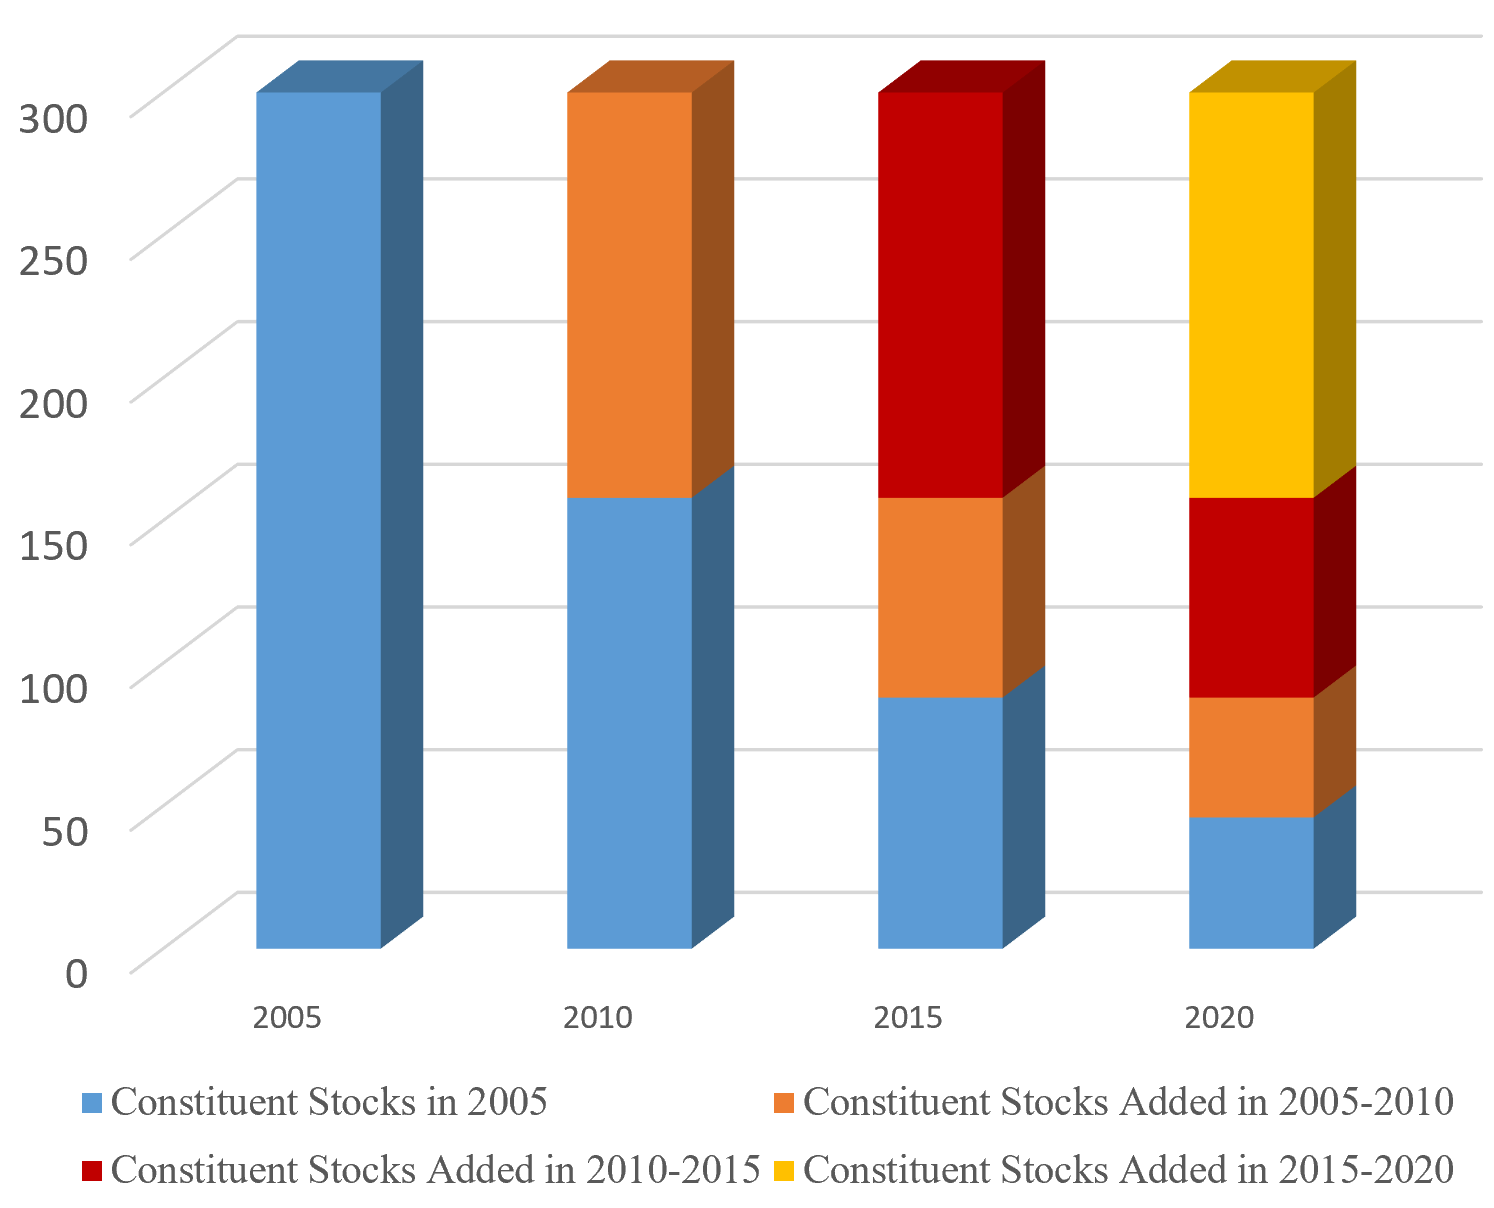
\includegraphics[width=\textwidth]{pic/CSI300.png}
        \caption{CSI 300}
    \end{subfigure}
    \begin{subfigure}[b]{0.5\textwidth}
        \centering
        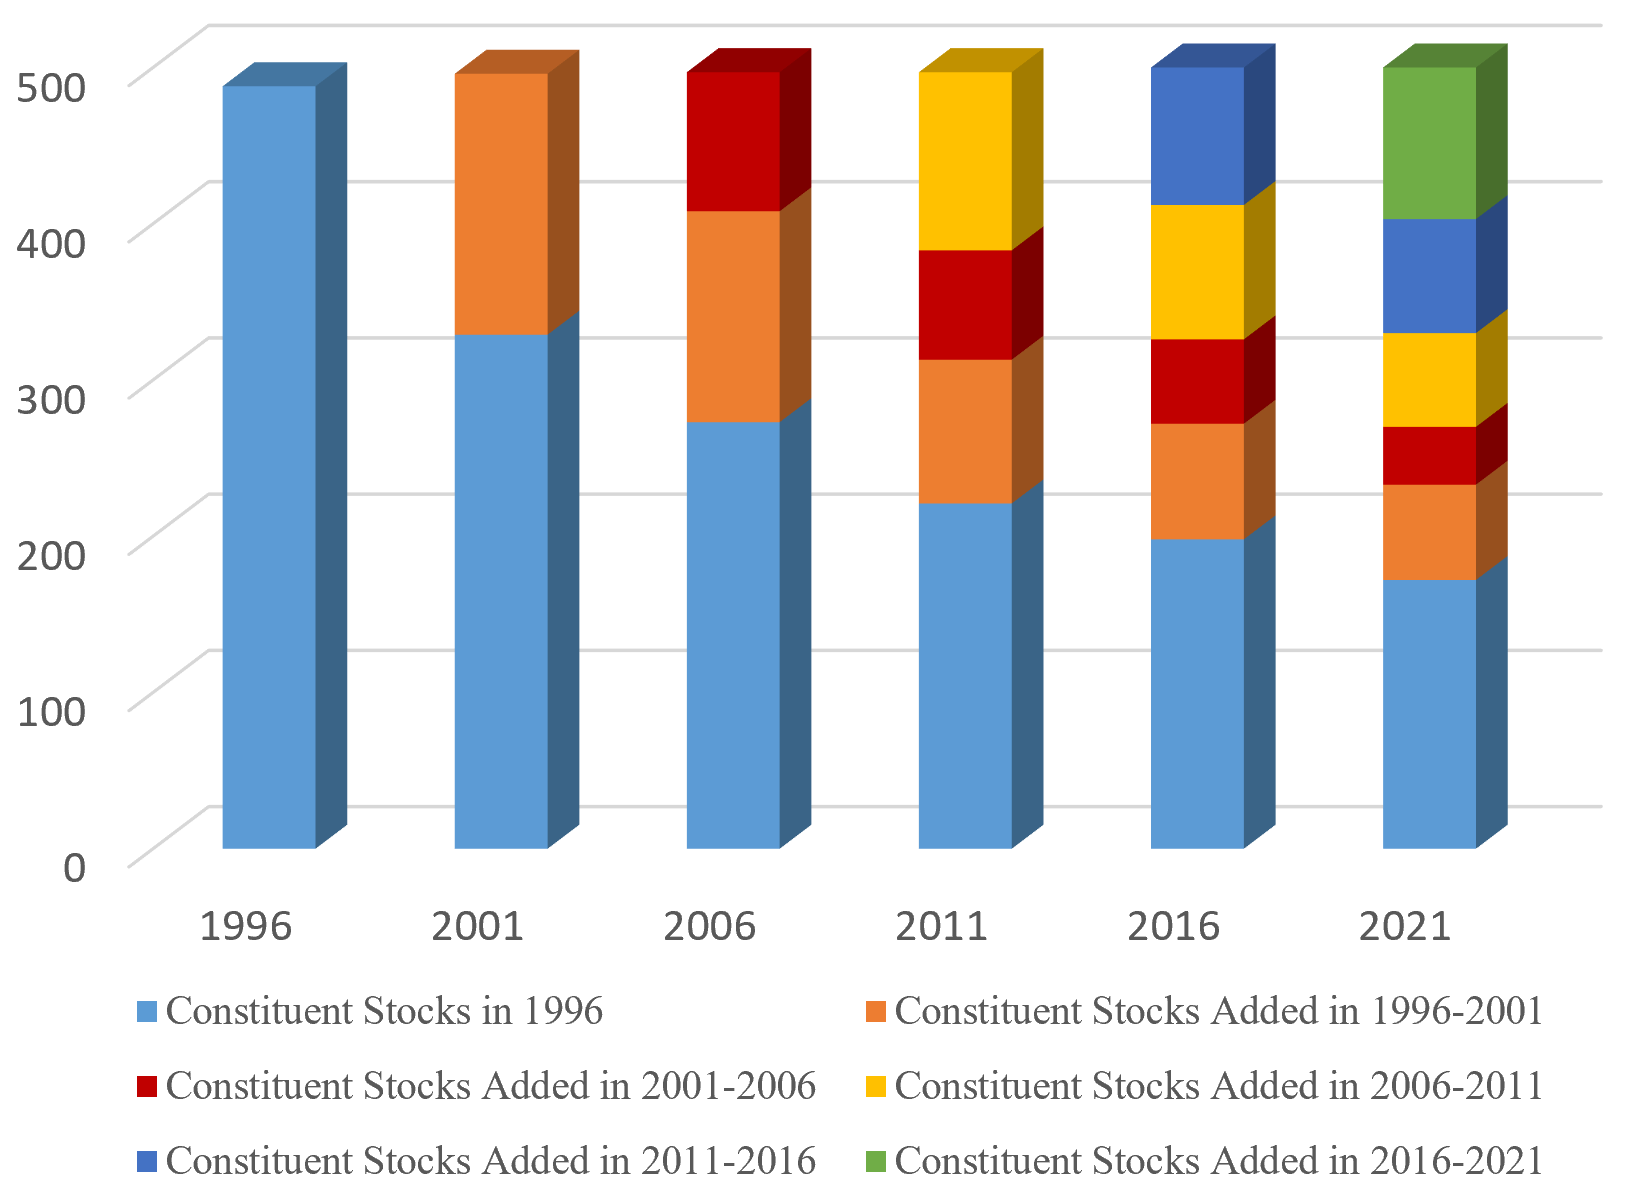
\includegraphics[width=\textwidth]{pic/S_P500.png}
        \caption{S\&P 500}
    \end{subfigure}
\caption{Historical retention status of CSI 300 and S\&P 500 constituent stocks}
\label{fig_CSI}
\end{figure}

Despite their empirical prevalence, theoretical work on dynamic spatial or network panels has overwhelmingly assumed balanced panels. \cite{KAPOOR200797} study the estimation of static spatial panel data models. %\cite{YU2008118}
\cite{YU2008118} and \cite{LeeSDPD} propose quasi-maximum likelihood estimation (QMLE) for spatial dynamic panel data models. \cite{LEE2014174} consider the generalized method of moments (GMM) estimation for spatial dynamic panel data. \cite{lee_qml_2012} and \cite{QU2017173} extend the previous spatial dynamic panel data to scenarios with time-varying or endogenous spatial weight matrices.
\cite{pmid32094164} propose a least squares estimators based on the eigendecomposition of a spatial weight matrix method for general spatial dynamic panel data models.
On this basis, \cite{HOU2024105605} extend this framework to directed networks and develop a variable selection approach for high-dimensional spatial dynamic panel data models. Another related model is the network autoregressive model. See \cite{10.1214/16-AOS1476} and \cite{ZHU2019345}. 
While these studies collectively enrich the methodological toolkit for dynamic spatial and network panel models, they all focus on balanced panel data settings.

In the field of unbalanced panel data, existing studies have focused on specific subtopics but lack integration with spatial dynamic structures. \cite{c50faaf4-3ca5-360a-914d-60311fe2980c}, \cite{1ade2690-c518-3924-afd9-60d7e947837b}, and \cite{HONORE2004293} address censored unbalanced panel data models, while \cite{WOOLDRIDGE1995115} and \cite{d0ceac3d-09ee-347a-9a49-b8b357c03f08} investigate unbalanced panels with sample selection bias. \cite{su_estimation_2025} develop estimation and inference methods for unbalanced panels with interactive fixed effects, and \cite{SASAKI2017320} study dynamic panel data with irregular time intervals. For spatial panel data, \cite{Meng21042026} examine a static genuinely unbalanced spatial panel data model, while \cite{Meng25072025} focus on static spatial panel data models with missing observations. None provide a unified framework for estimation and inference in unbalanced dynamic network panels.

This paper bridges this gap. We propose a quasi-maximum likelihood estimator (QMLE) for an unbalanced dynamic network panel model that captures network interactions and temporal dynamics simultaneously, while explicitly accommodating unit entry and exit.
We focus on panels that are \textit{genuinely} unbalanced \citep{Meng21042026}, \textbf{meaning that the unbalancedness is driven by the entry and exit of units rather than by missing observations}. This specification allows us to avoid modeling the missing-data process.
%By replacing lagged terms with a listing effect in a unit’s first active period, our model avoids the need to specify a missing-data mechanism.
Our main contributions and results are as follows.


\begin{enumerate}
\item We propose a baseline one-way fixed effect (OWFE) model for genuinely unbalanced dynamic network panels. The model incorporates contemporaneous network spillovers, lagged network and temporal effects, and a common listing
effect in a unit's first active period. For this model, we develop the QMLE, establish consistency and asymptotic normality, characterize the incidental-parameter bias, and derive a bias-corrected estimator with a consistent asymptotic covariance matrix estimator.

\item Since the size and elements of the network weight matrices vary over time, our setting differs from balanced spatial panel models. We establish new linear--quadratic form results that extend the existing theory from balanced spatial dynamic panels to genuinely unbalanced dynamic network panels. These results may also be useful for future studies of unbalanced network panel data.

\item We further extend the baseline framework to a two-way fixed effect (TWFE) specification. Under this extension, the QMLE remains consistent, while the incidental-parameter bias contains both the OWFE bias component and an additional component induced by the time fixed effects. We derive the corresponding asymptotic distribution, bias correction, and consistent asymptotic covariance matrix estimator.
\end{enumerate}


We examine the finite sample performance of the estimator through Monte Carlo simulations. Furthermore, we apply our model to study an empirical Airbnb listing dataset. We compare the estimated results across different regions and spatial scales to analyze the similarities and differences in the dynamic pricing behavior of Airbnb listings across cities.



The rest of the paper is organized as follows. Section~\ref{section2}
introduces the baseline OWFE model and the concentrated likelihood. Section~\ref{section3}
develops the asymptotic theory, bias correction, and covariance estimation for
the baseline QMLE. Section~\ref{sec:twoway_extension} extends the framework to
TWFE. Section~\ref{section4} reports Monte Carlo simulations, with additional
TWFE results provided in the appendix. Section~\ref{section5} presents the
empirical application, and Section~\ref{section6} concludes. All proofs are
collected in the Supplementary Appendices.


%This paper is organized as follows. In Section \ref{section2}, we introduce our model and derive the concentrated log-likelihood function. Section \ref{section3} establishes the consistency and asymptotic distribution of the QMLE. In addition, based on the asymptotic bias of the QMLE, we derive a bias-corrected estimator. Section \ref{section4} uses Monte Carlo simulations to examine the consistency and asymptotic normality of both the original QMLE and its bias-corrected counterpart. Section \ref{section5} presents an empirical evaluation of the model’s performance using real-world data. Section \ref{section6} concludes the paper. All proofs are collected in the appendices.

\section*{Notation}
We define $\iota_N$ as the $N$-dimensional column vector of ones, and $I_N$ as the $N$-dimensional identity matrix.
For any matrix $B$, $B_{ij}$ represents the $(i,j)$-th element of the matrix $B$. $B_{i,\cdot}$ and $B_{\cdot,j}$ are the $i$-th row and $j$-th column of $B$, respectively.
Denote $\|B\|_{1}\equiv\sup_{1\leq j\leq N}\sum_{i=1}^N|B_{ij}|$ and $\|B\|_{\infty}\equiv\sup_{1\leq i\leq N}\sum^N_{j=1}|B_{ij}|$ as the one-norm and the infinity-norm for matrix $B$, respectively. 
For a vector \(C\), let
\(\|C\|_1=\sum_{i=1}^N|C_i|\),
\(\|C\|_\infty=\sup_i|C_i|\), and
\(\|C\|_2=(\sum_{i=1}^N C_i^2)^{1/2}\)
denote the \(\ell_1\), infinity, and Euclidean norms of \(C\), respectively.
%For a vector $C$, denote $\|C\|_{1}=\sum_{i=1}^N|C_i|$, $\|C\|_{\infty}=\sup_i|C_i|$ and $\|C\|_2\equiv(\sum_{i=1}^N C_i^2)^{\frac{1}{2}}$ as the Euclidean norm of vector $C$.
Let $\mathrm{tr}(B)$ denote the trace of matrix $B$ and $|B|$ denote the determinant of $B$.
Define $\sup_t B_{t}$ as the element-wise supremum of the matrix sequence $\{B_{t}\}$, which means that $(\sup_t B_{t})_{ij}=\sup_t B_{t,ij}$ for $i,j=1,\cdots, N$.
Also, $\mathrm{abs}(B)$ represents the element-wise absolute value of the matrix $B$, i.e., $[\mathrm{abs}(B)]_{ij}=|B_{ij}|$.
For any square matrix $B$, $B^-$ denotes the strictly lower triangular part of $B$, obtained by setting the diagonal and upper triangular entries to zero.
The notation $\mathrm{diag}(b_1,\cdots, b_N)$ represents a diagonal matrix with diagonal entries $b_1,b_2,\cdots,b_N$.
Moreover, $\mathrm{blkdiag}(B_1,\cdots,B_T)$ forms a block-diagonal matrix by the given submatrices.
For brevity, the transposes of symmetrically positioned submatrices in a symmetric matrix are sometimes denoted by $*$.
$\mathrm{Var}$ and $\mathrm{Cov}$ represent the variance and covariance of random variables, respectively.







\section{The Model and Concentrated Likelihood Function}\label{section2}
\subsection{The Model}
Consider a genuinely unbalanced dynamic network panel, where nodes are fully observed during each period (i.e., there are no missing data), and nodes that are not listed do not have any impact on the whole network.
Suppose that we have observations for a network of $N$ nodes over $T$ time periods. 
%We can construct the spatial adjacency matrix $A$ of size $N\times N$ for the entire network based on the correlation between the nodes. 
However, for the $i$-th node, we only have a total of $T_i$ consecutive observations\footnote{
We assume that each individual enters the market only once. This condition can be generalized to allow the same individual to enter and exit multiple times.}. %The duration of each observed node cannot be aligned.
%The first and last observed times of each node are different, but the observations of each node are continuous, which means the observation on each nodes are equally spaced in time.
In the $t$-th time period, observed nodes may drop out of the network, and new nodes may join the network. We can only observe $N_t$ nodes in period $t$ and let $\mathbb{I}_t = \{i_1, i_2, \cdots, i_{N_t}\}$ denote the set of indices of nodes observed. Their corresponding attributes are $(y_{it},x_{it}')$ for each $i\in\mathbb{I}_t$, where $y_{it}$ is a scalar dependent variable and $x_{it}$ is a $k$-dimensional vector of regressors. The total sample size is $n=\sum_{t=1}^{T}N_t$.


%Assume for each nodes, the observation are continuous, which means the observation on each nodes are equally spaced.


Then we can establish the following model: for $t=1,2,\cdots,T$ and $i\in\mathbb{I}_t$,
\begin{align}\label{model_e}
y_{it}=\rho_0\sum_{j\in\mathbb{I}_t}w_{ij,t}y_{jt}+d_{i,t-1}(\lambda_0\sum_{j\in\mathbb{I}_{t-1}}m_{ij,t}y_{j,t-1}+\nu_0 y_{i,t-1})+d_{it}&(1-d_{i,t-1})\gamma_0+x_{it}'\beta_0+\alpha_{i0}+v_{it},
\end{align}
%$$y_{it}=\rho\sum_{j=1}^{N_t}w_{ij,t}y_{jt}+\lambda\sum_{j=1}^{N_{t-1}}m_{ij,t}y_{j,t-1}+\nu d_{i,t-1}y_{i,t-1}+d_{it}(1-d_{i,t-1})\gamma_{i}+x_{it}\beta+\alpha_i+v_{it},$$
%
%Model (\ref{model_e}) interpret $y_{i,t}$ as 
where $w_{ij,t}$ and $m_{ij,t}$ are predefined network weights,
%, they are normalized by restricting $\sum_{j=1}^{N_t}w_{t,ij}=1$ and $\sum_{j=1}^{N_t}m_{t,ij}=1$. 
and $d_{it}$ is an indicator that equals $1$ if $y_{it}$ is observed and 0 otherwise. $\gamma_0$ and $\alpha_{i0}$ are unknown listing and individual fixed effects, respectively, where the listing effect only takes effect at the first appearance of each individual, and the effect is identical for each individual. %\footnote{In fact, our model does not need to restrict each node to have consecutive observations. For nodes with intermittent observations, the listing effect is also activated whenever the node re-enters the network. For simplicity, we consider an unbalanced panel with consecutive observations in our theoretical analysis.}
%The above model assumes that $y_{it}$ is affected not only by its own factors and the network it is currently in, but also by the state at the last time. 
The above model assumes that $y_{it}$ is not only affected by its own covariates and the current network structure, but also by the fixed listing effect if node $i$ has just been listed or by its own lagged outcome and the lagged network state if node $i$ was already present. Since we only model the nodes that appear at $t = 0$ or later and cannot observe the data for $t<0$, to simplify the analysis, we ignore the impact of nodes that existed only before $t=0$.
%$\alpha_i$ is the unknown

Denote $Y_t=(y_{i_1t},\cdots,y_{i_{N_t}t})'$ as an $N_t$-dimensional column vector, $X_t=(x_{i_1t},\cdots,x_{i_{N_t}t})'$ as an $N_t\times k$ matrix, and $V_t=(v_{i_1t},\cdots,v_{i_{N_t}t})'$ as an $N_t$-dimensional column vector, where $i_1,\cdots,i_{N_t}\in\mathbb{I}_t$.
Define $\alpha_0=(\alpha_{10},\alpha_{20},\cdots,\alpha_{N0})'$. The $N_t\times N$ matrix $D_t$ is obtained by removing the rows corresponding to unobserved nodes during period $t$ from $I_N$.
%Noted that $D_t$
Then the above model can be written in the following matrix form: for $t=1,2,\cdots,T$,
\begin{align}\label{model_m}
Y_t=\rho_0 W_tY_t+\lambda_0 D_t(I_N-F_t)D_t'M_tY_{t-1}+\nu_0 D_tD_{t-1}'Y_{t-1}+\gamma_0 D_t F_t\iota_N+X_t\beta_0+D_t\alpha_0+V_t.
\end{align}
In the above model, $W_t$ and $M_t$ are $N_t \times N_t$ and $N_t \times N_{t-1}$ network weight matrices, respectively. The elements of $W_t$ and $M_t$ are defined as:  
$$
(W_t)_{k,l} \equiv w_{i_ki_l,t}, \quad \text{for } k,l=1,2,\cdots,N_t \text{ and } i_k,i_l\in\mathbb{I}_t,
$$  
$$
(M_t)_{k,l} \equiv m_{i_kj_l,t}, \quad \text{for } k=1,2,\cdots,N_t\text{, }l=1,2,\cdots,N_{t-1}\text{, }  i_k\in\mathbb{I}_t\text{ and } j_l\in\mathbb{I}_{t-1}.
$$  
%非随机 Xit, 结构, 弱相关
%New Zealand: xining, auckland


%where \textcolor{blue}{$W_t=\left(w_{ij,t}|i,j\in\mathbb{I}_t\right)$ and $M_t=\left(m_{ij,t}|i\in\mathbb{I}_t,j\in\mathbb{I}_{t-1}\right)$} are the $N_t\times N_t$ and $N_t\times N_{t-1}$ spatial weight matrices.
%consist of $\{w_{ij,t}|i,j\in\mathbb{I}_t\}$ and $\{m_{ij,t}|i\in\mathbb{I}_t,j\in\mathbb{I}_{t-1}\}$ respectively, which can be obtained by row-normalizing $D_tAD_t'$ and $D_tAD_{t-1}'$, respectively.  
The $N$-dimensional diagonal matrix $F_t\equiv D_t'D_t(I_N-D_{t-1}'D_{t-1})=\mathrm{diag}(d_{1t}(1-d_{1,t-1}),\cdots,$ $d_{N,t}(1-d_{N,t-1}))$ is the listing index matrix. $F_t\iota_N$ is sparser than other covariates because, over all $T$ periods, fewer than $N$ individuals can newly join the network.

Let \(S_t\equiv I_{N_t}-\rho_0W_t\), which is assumed to be invertible, and define
\(A_t\equiv D_t[\lambda_0(I_N-F_t)D_t'M_t+\nu_0D_{t-1}']S_{t-1}^{-1}\).
Assume that the following infinite summation is well-defined. Then repeated substitution of model~(2) gives
\begin{align}
Y_t&=\sum_{h=0}^{\infty}S_{t}^{-1}A_t^{(h)}[D_{t-h} (\gamma_0F_{t-h}\iota_N+\alpha_0)+X_{t-h}\beta_0+V_{t-h}]\equiv\mathcal{E}_t+\mathcal{X}_t\beta_0+\mathcal{V}_t,\label{model_sumV}
\end{align}
where $A_t^{(h)}\equiv A_{t}A_{t-1}\cdots A_{t-h+1}$ for $h=1,2,\cdots$ and $A_t^{(0)}\equiv I_{N_t}$, $\mathcal{E}_t\equiv \sum_{h=0}^{\infty}S_{t}^{-1}A_t^{(h)}D_{t-h}(\gamma_0F_{t-h}\iota_N+\alpha_0)$, 
%$\mu_\alpha\equiv \sum_{h=0}^{\infty}A_t^{(h)}S_{t-h}^{-1}D_{t-h}\alpha_0$, 
$\mathcal{X}_t\equiv \sum_{h=0}^{\infty}S_{t}^{-1}A_t^{(h)}X_{t-h}$ and $\mathcal{V}_t\equiv \sum_{h=0}^{\infty}S_{t}^{-1}A_t^{(h)}V_{t-h}$. 
The above decomposition can be viewed as an infinite moving average representation of $Y_t$. 
%From the above decomposition, $Y_t$ can be viewed as an infinite moving average representation. 
We establish the law of large numbers and the central limit theorem based on this decomposition in the lemmas in Supplementary Appendix A.




%Similarly, $F_t$ denotes the listing index matrix and is obtained by keeping only the corresponding rows of nodes that first appear during period $t$.
%and $F_t$ denotes the $N_t\times N$ indicator 



\subsection{Quasi-Maximum Likelihood Method}
Define $Z_t\equiv(D_t(I_N-F_t)D_t'M_tY_{t-1},D_tD_{t-1}'Y_{t-1},D_tF_t\iota_N,X_t)$, $\delta_0\equiv(\lambda_0,\nu_0,\gamma_0,\beta_0')'$.
%where we scale both $\gamma$ and its covariate by $\sqrt{T}$ respectively to ensure unified asymptotic analysis. 
Then model (\ref{model_m}) can be simplified to
\begin{align}\label{model_simp}
Y_t=\rho_0 W_tY_t+ Z_t\delta_0+D_t\alpha_0+V_t.
\end{align}
Stacking the matrices and vectors in model (\ref{model_simp}) for $t=1,2,\cdots,T$, we have 
\begin{align}\label{model_acc}
\mathbb{Y}=\rho_0\mathbb{W}\mathbb{Y}+\mathbb{Z}\delta_0+\mathbb{D}\alpha_0+\mathbb{V},
\end{align}
where $\mathbb{Y}=(Y_1',\cdots,Y_T')'$, $\mathbb{W}=\mathrm{blkdiag}(W_1,\cdots,W_T)$, $\mathbb{Z}=(Z_1',\cdots,Z_T')'$, $\mathbb{D}=(D_1',\cdots,D_T')'$ and $\mathbb{V}=(V_1',\cdots,V_T')'$.
Note that $\mathbb{D'D}=\sum_{t=1}^TD_t'D_t=\sum_{t=1}^T\mathrm{diag}(d_{1t},d_{2t},\cdots,d_{N,t})=\mathrm{diag}(T_1,T_2,\cdots,T_N)\equiv\mathcal{T}$.
Assume $v_{it}$ are i.i.d. random variables with mean $0$ and variance $\sigma^2_0$. Denote the parameters of interest as $\theta=(\rho,\delta',\sigma^2)'$ and let $\zeta=(\rho,\delta')$. Then the log-likelihood function of model (\ref{model_acc}) is
\begin{align}\label{MLE}
L_n(\theta,\alpha)=-\frac{n}{2}\ln2\pi-\frac{n}{2}\ln\sigma^2+\ln|\mathbb{S}(\rho)|-\frac{1}{2\sigma^2}\mathbb{V}'(\zeta,\alpha)\mathbb{V}(\zeta,\alpha),
\end{align}
where $\mathbb{S}(\rho)\equiv I_{n}-\rho\mathbb{W}$ and $\mathbb{V}(\zeta,\alpha)\equiv\mathbb{S(\rho)Y-Z}\delta-\mathbb{D}\alpha$. Given $\zeta$, $L_n(\theta,\alpha)$ is maximized at
$\hat{\alpha}(\zeta)=\mathbb{(D'D)}^{-1} \mathbb{D'}(\mathbb{S}(\rho)\mathbb{Y-Z\delta)}$.
Substituting $\hat{\alpha}$ into (\ref{MLE}), we obtain our 
estimator $\hat{\theta}$ by maximizing the following concentrated log-likelihood function
\begin{equation}
L_n^c(\theta)=-\frac{n}{2}\ln2\pi-\frac{n}{2}\ln\sigma^2+\ln|\mathbb{S}(\rho)|-\frac{1}{2\sigma^2}\widetilde{\mathbb{V}}'(\zeta)\widetilde{\mathbb{V}}(\zeta),\label{CMLE}
\end{equation}
where $\widetilde{\mathbb{V}}(\zeta)\equiv\mathbb{S}(\rho)\mathbb{Y-Z\delta}-\mathbb{D}\hat{\alpha}(\zeta)=\mathbb{Q(S(\rho)Y-Z\delta})$ and $\mathbb{Q}\equiv I_{n}-\mathbb{P}$, $\mathbb{P}\equiv\mathbb{D}(\mathbb{D}'\mathbb{D})^{-1}\mathbb{D}'$.
Moreover, the corresponding expected value function of $L_n^c(\theta)$ is
\begin{align}
Q_n(\theta)\equiv E[L_n^c(\theta)]=-\frac{n}{2}\ln2\pi-\frac{n}{2}\ln\sigma^2+\ln\left|\mathbb{S}(\rho)\right|-\frac{1}{2\sigma^2}E\left[\widetilde{\mathbb{V}}'(\zeta)\widetilde{\mathbb{V}}(\zeta)\right].\label{eq_Q_n}
\end{align}
We derive the asymptotic properties of the estimators based on $L_n^c(\theta)$ and $Q_n(\theta)$. In practice, we further concentrate out $\delta$ and $\sigma^2$ to accelerate computation, that is, we optimize $$L_{n}^{cc}(\rho)\equiv-\frac{n}{2}\ln2\pi-\frac{n}{2}\ln\hat{\sigma}^2+\ln|\mathbb{S}(\rho)|-\frac{n}{2}$$ instead, where
$\hat{\delta}(\rho)
=\left(\mathbb{Z}'\mathbb{Q}\mathbb{Z}
\right)^{-1}\mathbb{Z}'\mathbb{Q}\mathbb{S}(\rho)\mathbb{Y},$ and
$\hat{\sigma}^2(\rho)=\frac{1}{n}\mathbb{Y'S(\rho)}'[\mathbb{Q}-\mathbb{QZ(Z'QZ})^{-1}\mathbb{Z'Q}]\mathbb{S(\rho)Y}$.


\section{Asymptotic properties of QMLE}\label{section3}
\subsection{Consistency of QMLE}
%Since the listing effect $\gamma$ appears in the model fewer than $N$ times, its convergence rate is intuitively slower than that of the other parameters. 
In the proof of consistency, we first establish the consistency of all parameters except $\gamma$, and then prove the consistency of $\gamma$.
Define $\mathbb{Z}^{(-\gamma)}$ as the matrix obtained by removing the third column from $\mathbb{Z}$, and let $\mathbb{Z}^{(\gamma)}$ be the third column of $\mathbb{Z}$.
The following assumptions are needed for consistency.

\begin{assumption}\label{asp_2}
The unbalancedness of the model is nonstochastic, which means that $d_{it}$ and $D_t$ are nonstochastic for all $i$ and $t$. %$\sum_{i=1}^N \frac{T}{T_i}=O(N)$.
There is a lower bound on the number of observations for all individuals, i.e., $T_i\geq c_T T$ for all $i$, where $c_T>0$ is a constant that does not vary with $N$ or $T$. 
Additionally, $N_0<c_NN$, where $N_0$ denotes the number of units observed at $t=0$ and $0<c_N<1$ is a constant that does not vary with $N$ or $T$.
\end{assumption}
\begin{assumption}\label{asp_error}
The error terms $v_{it}$ are i.i.d. across $i$ and $t$ with mean 0, variance $\sigma^2_0$, third moment \(\mu_3\) and fourth moment \(\mu_4\). $E|v_{it}|^{4+2\eta}<\infty$ for some $\eta>0$. %Assume $E(v_{it}|\alpha_i)=0$.
\end{assumption}
%\begin{assumption}\label{asp_alpha}\textcolor{red}{The fixed effect $\alpha_i$ are independent and $E(\alpha_i)<\infty$, $\mathrm{Var}(\alpha_i)<\infty$ uniformly for $i$.}\end{assumption}
\begin{assumption}\label{asp_4}
$\sup_{\rho\in\Lambda}\sup_{N,T}\sup_t\|\rho W_t\|_{\infty}<1$, where $\Lambda$ is the parameter space of $\rho$. Moreover, $\Lambda$ is compact and $\rho_0$ lies in the interior of $\Lambda$.
\end{assumption}

\begin{assumption}\label{asp_X}
The elements of $x_{it}$ and $\alpha_{i0}$ are nonstochastic and bounded uniformly in $i$, $t$, $N$ and $T$. $\mathbb{Z'QZ}$ is nonsingular. Also, $\lim_{n\rightarrow\infty}\frac{1}{n}E(\mathbb{Z}^{(-\gamma)\prime}\mathbb{QZ}^{(-\gamma)})$ exists and is nonsingular, where $n=\sum_{t=1}^{T}N_t$ is the total sample size.
\end{assumption}

\begin{assumption}\label{asp_UB}
The sequences of matrices $\{W_t\}$, $\{M_t\}$ and $\{S_t^{-1}\}$ are nonstochastic and uniformly bounded in row and column sum norms (for short, UB)
\footnote{We say a $N\times N$ matrix $B$ is UB if $\sup_{N}\max\{\|B\|_1,\|B\|_\infty\}<\infty$. We say a sequence of $N_t\times N_t$ matrices $\{B_{t}\}$ is UB uniformly for $t$ if $\sup_{N,T}\sup_t\max\{\|B_{t}\|_1,\|B_{t}\|_\infty\}<\infty$.}
uniformly for $t$. Moreover,$$\max(\|\sup_t \mathrm{abs}(D_t'S_t^{-1}D_t)\|_\infty,\|\sup_t \mathrm{abs}(D_t'W_tD_t)\|_\infty,\|\sup_t \mathrm{abs}(D_t'M_tD_{t-1})\|_\infty)<\infty.$$
\end{assumption}
\begin{assumption}\label{asp_UBA}
$\sum_{h=1}^{\infty}\mathrm{abs}\left(D_t'A_{t}^{(h)}D_{t-h}\right)$ and $\sum_{h=t}^{\infty}\mathrm{abs}\left(D_h'A_{h}^{(h-t)}D_t\right)$ are UB uniformly for $t$.
%\textcolor{cyan}{Assume $\sum_{h=1}^{\infty}\mathrm{abs}\left(\mathcal{A}_{t}^{(h)}\right)$ and $\sum_{h=t}^{\infty}\mathrm{abs}\left(\mathcal{A}_{h}^{(h-t)}\right)$ are \rm{UB} uniformly for $t$}.
\end{assumption}
\begin{assumption}\label{asp_n}
$N$ is a nondecreasing function of $T$, and $N$ will go to infinity as $T$ goes to infinity.
\end{assumption}

%Assumption \ref{asp_W} is a standard normalization assumption in spatial econometrics. 
Assumption \ref{asp_2} regulates the unbalancedness of the panel, where we assume the unbalancedness to be nonstochastic. We will leave the more complicated case where $d_{it}$ is stochastic for future research. 
%where the assumption on $T_i$'s imposed to control the asymptotic bias of the estimator. This condition requires that the majority of $T_i$'s be of the same order as $T$, while allowing a finite number of $T_i$'s to be of order $O(\frac{T}{N})$.
A lower bound on $T_i$ is imposed to ensure the consistency of the estimator for $\alpha$, and an upper bound on $N_0$ is imposed to guarantee the consistency of the estimator for $\gamma$, as it requires sufficiently many observed listing effects. If this condition is not satisfied, a similar asymptotic analysis can still be conducted, but the convergence rate of $\hat{\gamma}$ will change.
%Moreover, the upper bound of $N_0$ is imposed to guarantee the consistency of the estimator for $\gamma$, as it requires sufficiently many observed listing effects.
Assumption \ref{asp_error} provides regularity assumptions for $v_{it}$. %The existence of moments of order greater than fourth is required to derive the central limit theorem in Supplementary Appendix A, Lemma 18. 
Similar assumptions are adopted in \cite{https://doi.org/10.1111/j.1468-0262.2004.00558.x} and \cite{YU2008118}. Assumption \ref{asp_4} is a standard assumption for spatial (or network) panel data models. It implies that $S_t(\rho)^{-1}$ exists and
\begin{align}
\sup_{\rho\in\Lambda}\sup_{N,T}\sup_t\|S_t(\rho)^{-1}\|_{\infty}<\infty,\label{eq_asp_S}
\end{align}
which is proved in equation (S.28) in the supplementary materials of \cite{Wu_Jiang_Xu_2024}.
Although the assumption that $\rho_0$ lies in the interior of the parameter space is in fact imposed for simplicity and not required for consistency, we state the conditions jointly for notational convenience.
Assumption \ref{asp_X} rules out multicollinearity, ensuring that $\delta$ is estimable.
We consider fixed design in this paper as in \cite{https://doi.org/10.1111/j.1468-0262.2004.00558.x,LEE2007489}, \cite{YU2008118} and \cite{LEE2014174}, among others. This assumption can be relaxed to allow for stochastic exogenous variables by using the near-epoch dependence theory in \cite{JENISH2012178} or the functional dependence theory in \cite{Wu_Jiang_Xu_2024}. The proof is similar to the proof under fixed design. 
Assumption \ref{asp_UB} is a standard condition in the literature of spatial and network econometrics. See \cite{https://doi.org/10.1111/j.1468-0262.2004.00558.x,LEE2007489}, \cite{YU2008118} and \cite{LEE2014174}. The assumption that $\sup_{N,T}\sup_t\|S_t^{-1}\|_\infty<\infty$ can in fact be ensured by equation (\ref{eq_asp_S}).
Moreover, Assumption \ref{asp_UB} implies that $\{S_{t}(\rho)^{-1}\}$ is UB uniformly in a neighborhood of $\rho_0$, from Lemma A.3 of \cite{https://doi.org/10.1111/j.1468-0262.2004.00558.x}.
Assumption \ref{asp_UBA} restricts the joint effect of network spillovers and temporal dynamics, which is a common assumption in dynamic network panel data, such as Assumption 6 in \cite{YU2008118}, Assumption 7 in \cite{LEE2014174} and Assumption 6 in \cite{lee_qml_2012}. 
Assumptions \ref{asp_UB} and \ref{asp_UBA} are imposed to establish a law of large numbers and a central limit theorem for certain quadratic forms of the network lag spillover term $M_tY_{t-1}$ and the temporal lag term $Y_{t-1}$.
Assumption \ref{asp_n} means that we consider a large-$N$ and large-$T$ setting, in which the QMLE is consistent. For short dynamic network panel data models, other estimation methods, such as GMM, are required.

Denote $\mathbb{S}_0\equiv\mathbb{S}(\rho_0)$, $\mathbb{G}(\rho)\equiv\mathbb{WS}(\rho)^{-1}$ and $\mathbb{G}_0\equiv\mathbb{WS}^{-1}_0$. Define $\mathcal{H}^{(-\gamma)}\equiv\frac{1}{n}(\mathbb{G}_0\mathbb{Z}\delta_0+\mathbb{G}_0\mathbb{D}\alpha_0,\mathbb{Z}^{(-\gamma)})'\mathbb{Q}(\mathbb{G}_0\mathbb{Z}\delta_0+\mathbb{G}_0\mathbb{D}\alpha_0,\mathbb{Z}^{(-\gamma)})$ and  $\sigma_n^2\equiv\allowbreak\frac{\sigma^2_0}{n}tr[(\mathbb{S(\rho)S}_0^{-1})'\mathbb{S(\rho)S}_0^{-1}]$. As in \cite{YU2008118}, the following assumption is needed to establish the global identification condition required for consistency.
\begin{assumption}\label{asp_EH}%\label{asp_Vari}
At least one of the following two conditions is satisfied: (i) $\lim_{n\rightarrow\infty}E\mathcal{H}^{(-\gamma)}$ exists and is nonsingular.
(ii) $\lim_{n\rightarrow\infty}\left(\frac{1}{n}\ln|\sigma_0^2\mathbb{S}_0^{-1}\mathbb{S}_0^{-1\prime}|-\frac{1}{n}\ln|\sigma_n^2\mathbb{S}(\rho)^{-1}\mathbb{S}(\rho)^{-1\prime}|\right)\neq0$ for $\rho\neq\rho_0$.
\end{assumption}

%Denote $\Gamma=\mathrm{blkdiag}(I_3,\sqrt{T},I_{k+1})$ and $\widetilde{\Gamma}=\mathrm{blkdiag}(I_2,\sqrt{T},I_k)$. Define $\mathcal{H}\equiv\frac{1}{n}\Gamma'(\mathbb{G}_0\mathbb{Z}\delta_0,\mathbb{Z})'\mathbb{Q}(\mathbb{G}_0\mathbb{Z}\delta_0,\mathbb{Z})\Gamma$\textcolor{blue}{, where the $\sqrt{T}$-scaling the covariate term of $\gamma_0$ ensures unified convergence rates in asymptotic analysis.}
\begin{theorem}\label{consistency}
Under Assumptions \ref{asp_2}-\ref{asp_EH}, $\hat{\theta}\stackrel{p}{\rightarrow}\theta_0$.
\end{theorem}

%$\mathbb{Y}=\mathbb{S}(\rho)_0^{-1}(\mathbb{Z}\delta_0+\mathbb{D}\alpha_0+\mathbb{U})$
%\begin{align*}\ln L(\rho,\delta,\phi,\sigma^2)=-\sum_{t=1}^{T}\left(\frac{N_t}{2}\ln2\pi+\frac{N_t}{2}\ln\sigma^2-\ln|S_t|+\frac{1}{2\sigma^2}V_t'(\rho,\delta,\phi)V_t(\rho,\delta,\phi)\right),\end{align*}

\subsection{Asymptotic Distribution of QMLE}\label{section3.2}
Since we have concentrated out the $N$ individual fixed effects from the log likelihood function, the QMLE is subject to the incidental parameters problem, which induces an asymptotic bias in the estimator \citep{Meng21042026}.
We derive the asymptotic distribution of $\hat{\theta}$ by performing a Taylor expansion of $\frac{\partial L_n^c(\hat{\theta})}{\partial\theta}$ around $\theta_0$. The first and second order derivatives of $L_n^c(\theta)$ are derived in Supplementary Appendix  B.
According to (\ref{model_sumV}), denote $Z^\circ_t\equiv\left(D_t(I_N-F_t)D_t'M_t\mathcal{V}_{t-1},D_tD_{t-1}'\mathcal{V}_{t-1},\mathbf{0}_{N_t\times(k+1)}\right)$ and $\mathbb{Z}^\circ\equiv(Z^{\circ\prime}_1,\cdots,Z^{\circ\prime}_T)'$.
We decompose $\mathbb{QZ}$ into $\mathbb{QZ}=\widetilde{\mathbb{Z}}^{*}-\widetilde{\mathbb{Z}}^{\circ}$, where $\widetilde{\mathbb{Z}}^{\circ}\equiv\mathbb{P}\mathbb{Z}^{\circ}$ and $\widetilde{\mathbb{Z}}^{*}=\mathbb{QZ}+\widetilde{\mathbb{Z}}^{\circ}$.
Note that $Z_t^\circ$ is independent of $V_s$ when $t\leq s$, and $\widetilde{\mathbb{Z}}^{*}=\mathbb{QZ}+\widetilde{\mathbb{Z}}^{\circ}=\mathbb{Q(Z-Z}^\circ)+\mathbb{Z}^\circ$, where $\mathbb{Z-Z}^\circ$ is nonstochastic.
Decompose $\widetilde{\mathbb{Z}}^{*}$ into $N_t$-dimensional vectors $\widetilde{Z}_1^*,\cdots,\widetilde{Z}_T^*$ such that $\widetilde{\mathbb{Z}}^{*}=(\widetilde{Z}_1^{*\prime},\cdots,\widetilde{Z}_T^{*\prime})'$. Therefore, $\widetilde{Z}_t^{*}$ is independent of $V_s$ when $t\leq s$. But $\widetilde{\mathbb{Z}}^{\circ}$ is correlated with $\mathbb{V}$, as proved in Lemma 11 in Supplementary Appendix A.


Similarly, we can decompose $\mathbb{QG}_0\mathbb{Z}=\widetilde{\mathbb{G}_0\mathbb{Z}}^{*}-\widetilde{\mathbb{G}_0\mathbb{Z}}^{\circ}$, where
$\widetilde{\mathbb{G}_0\mathbb{Z}}^{\circ}\equiv\mathbb{P}\mathbb{G}_0\mathbb{Z}^{\circ}$ and $\widetilde{\mathbb{G}_0\mathbb{Z}}^{*}=\mathbb{QG}_0\mathbb{Z}+\widetilde{\mathbb{G}_0\mathbb{Z}}^{\circ}$. Further, decompose $\widetilde{\mathbb{G}_0\mathbb{Z}}^{*}$ into $N_t$-dimensional vectors $\widetilde{GZ}_1^*,\cdots,\widetilde{GZ}_T^*$ such that $\widetilde{\mathbb{G}_0\mathbb{Z}}^{*}=(\widetilde{GZ}_1^{*\prime},\cdots,\widetilde{GZ}_T^{*\prime})'$. Similarly, $\widetilde{GZ}_t^{*}$ is independent of $V_s$ when $t\le s$, whereas $\widetilde{\mathbb{G}_0\mathbb{Z}}^{\circ}$ is correlated with $\mathbb{V}$.

Let $\Gamma=\mathrm{blkdiag}(I_3,\sqrt{T},I_{k+1})$ and $\widetilde{\Gamma}=\mathrm{blkdiag}(I_2,\sqrt{T},I_{k})$. Then we can rewrite $\frac{1}{\sqrt{n}}\Gamma\frac{\partial L_n^c(\theta_0)}{\partial\theta}=\frac{1}{\sqrt{n}}\Gamma\frac{\partial L_n^{c*}(\theta_0)}{\partial\theta}-\Delta_n$, where
$$\frac{1}{\sqrt{n}}\Gamma\frac{\partial L_n^{c*}(\theta_0)}{\partial\theta}=\left(\begin{aligned}
&\frac{1}{\sqrt{n}\sigma^2_0}(\mathbb{G}_0\mathbb{D\alpha}_0)'\mathbb{QV}+\frac{1}{\sqrt{n}\sigma_0^2}\mathbb{V}'\mathbb{G}_0\mathbb{V}+\frac{1}{\sqrt{n}\sigma_0^2}(\widetilde{\mathbb{G}_0\mathbb{Z}}^*\delta_0)'\mathbb{V}-\frac{1}{\sqrt{n}}\mathrm{tr}(\mathbb{G}_0)\\
&\frac{1}{\sqrt{n}\sigma_0^2}\widetilde{\Gamma}\widetilde{\mathbb{Z}}^{*\prime}\mathbb{V}\\
&-\frac{n}{2\sqrt{n}\sigma_0^2}+\frac{1}{2\sqrt{n}\sigma_0^4}\mathbb{V'V}
\end{aligned}\right),$$
and
$$\Delta_n=\left(\begin{aligned}
&\frac{1}{\sqrt{n}\sigma_0^2}\mathbb{V}'\mathbb{G}_0'\mathbb{P}\mathbb{V}+\frac{1}{\sqrt{n}\sigma_0^2}(\widetilde{\mathbb{G}_0\mathbb{Z}}^\circ\delta_0)'\mathbb{V}\\
&\frac{1}{\sqrt{n}\sigma_0^2}\widetilde{\Gamma}\widetilde{\mathbb{Z}}^{\circ\prime}\mathbb{V}\\
&\frac{1}{2\sqrt{n}\sigma_0^4}\mathbb{V'}\mathbb{P}\mathbb{V}
\end{aligned}\right).$$
This decomposes $\frac{\partial L_n^c(\theta_0)}{\partial\theta}$ into two components: a mean zero term $\frac{\partial L_n^{c*}(\theta_0)}{\partial\theta}$ and a nonzero mean term $\Delta_n$. $\Delta_n$ can be regarded as the source of asymptotic bias arising from the estimation of fixed effects.
As derived in Supplementary Appendix B.2, $$E\left(\frac{1}{\sqrt{n}}\Gamma\frac{\partial L_n^{c*}(\theta_0)}{\partial\theta}\cdot\frac{1}{\sqrt{n}}\frac{\partial L_n^{c*}(\theta_0)}{\partial\theta'}\Gamma\right)=\Gamma\Sigma_{\theta_0,n}\Gamma+\Gamma\Omega_{\theta_0,n}\Gamma+O\left(\frac{1}{T}\right).$$
Denote $\Sigma_{\theta_0}\equiv\lim_{n\rightarrow\infty}\Gamma\Sigma_{\theta_0,n}\Gamma$, $\Omega_{\theta_0}\equiv\lim_{n\rightarrow\infty}\Gamma\Omega_{\theta_0,n}\Gamma$, then
\begin{align}
\lim_{n\rightarrow\infty}E\left(\frac{1}{\sqrt{n}}\Gamma\frac{\partial L_n^{c*}(\theta_0)}{\partial\theta}\cdot\frac{1}{\sqrt{n}}\frac{\partial L_n^{c*}(\theta_0)}{\partial\theta'}\Gamma\right)=\Sigma_{\theta_0}+\Omega_{\theta_0}.\label{eq_varg}
\end{align}

The asymptotic distribution of $\frac{\partial L_n^{c*}(\theta_0)}{\partial\theta}$ can be derived by applying the central limit theorem for martingale difference sequences, as proved in Lemma 18 in Supplementary Appendix A.
Furthermore, as derived in Supplementary Appendix B.4, we have $\Delta_n=\sqrt{\frac{N}{c_uT}}\varphi_n(\theta_0)+O_p\left(\frac{1}{\sqrt{T}}\right)$, where $c_u\equiv\frac{n}{NT}$, $\varphi_n(\theta_0)=O(1)$ and $\varphi_n(\theta)$ is defined in equation (B.6) in Supplementary Appendix B.4.

%Assumption \ref{asp_EH} ensures the nonsingularity of the information matrix $\Sigma_{\theta_0}$. If Assumption \ref{asp_EH} does not hold, the following assumption serves as an alternative.
The following assumption ensures the nonsingularity of the information matrix $\Sigma_{\theta_0}$.
\begin{assumption}\label{asp_nonsingularity} At least one of the following two conditions is satisfied: (i) $\lim_{n\rightarrow\infty}E\mathcal{H}^{(-\gamma)}$ exists and is nonsingular.
(ii) $\lim_{n\rightarrow\infty}\frac{1}{n}\left(\mathrm{tr}(\mathbb{G}_0^2+\mathbb{G}_0'\mathbb{G}_0)-\frac{2}{n}\left[\mathrm{tr}(\mathbb{G}_0)\right]^2\right)\neq0$.
\end{assumption}
%Assumption \ref{asp_nonsingularity} is imposed , as proved in Appendix \ref{B.3}.

\begin{theorem}\label{Normality}
Under Assumptions \ref{asp_2}-\ref{asp_nonsingularity},
\begin{align}
\sqrt{n}\Gamma^{-1}\left[\hat{\theta}-\left(\theta_0-\frac{\Sigma_{\theta_0,n}^{-1}\varphi_n(\theta_0)}{c_uT}\right)\right]+O_p\left(\max\left\{\frac{1}{\sqrt{T}},\sqrt{\frac{N}{T^3}}\right\}\right)\overset{d}{\rightarrow}N\left(0,\Sigma_{\theta_0}^{-1}(\Sigma_{\theta_0}+\Omega_{\theta_0})\Sigma_{\theta_0}^{-1}\right),\label{eq_Normality}
\end{align}
where $\Sigma_{\theta_0,n}^{-1}\varphi_n(\theta_0)$ is O(1).
\end{theorem}

If error terms $v_{it}$ are normal, $\Omega_{\theta_0}=0$ and the asymptotic variance of equation (\ref{eq_Normality}) becomes $\Sigma_{\theta_0}^{-1}$.
Theorem \ref{Normality} shows that $\hat{\theta}$ exhibits an asymptotic bias $-\Sigma_{\theta_0,n}^{-1}\varphi_n(\theta_0)/(c_uT)$. It also shows that $\hat{\theta}^{(-\gamma)}$ is $\sqrt{n}$-consistent and $\hat{\gamma}$ is $\sqrt{c_uN}$-consistent.
When $N/T\rightarrow0$, $\hat{\theta}$ is consistent and asymptotically centered normal, which means
$\sqrt{n}\Gamma^{-1}\left(\hat{\theta}-\theta_0\right)\overset{d}{\rightarrow}N\left(0,\Sigma_{\theta_0}^{-1}(\Sigma_{\theta_0}+\Omega_{\theta_0})\Sigma_{\theta_0}^{-1}\right)$.
%When $N/T\rightarrow c_{N/T}<\infty$, $\hat{\theta}$ is consistent and asymptotically normal, but not centered around 0, which means
%$$\sqrt{n}\Gamma^{-1}\left(\hat{\theta}-\theta_0\right)+\sqrt{c_{N/T}}c_u^{-1}\Gamma^{-1}\Sigma_{\theta_0,n}^{-1}\varphi_n(\theta_0)\overset{d}{\rightarrow}N\left(0,\Sigma_{\theta_0}^{-1}(\Sigma_{\theta_0}+\Omega_{\theta_0})\Sigma_{\theta_0}^{-1}\right).$$
%When $N/T\rightarrow\infty$, Theorem \ref{Normality} only indicates the consistency of $\hat{\theta}$, which means
%$$\sqrt{c_u}T\Gamma^{-1}\left(\hat{\theta}-\theta_0\right)+c_u^{-1}\Gamma^{-1}\Sigma_{\theta_0,n}^{-1}\varphi_n(\theta_0)\overset{p}{\rightarrow}0.$$

%we have $$\sqrt{n}\Gamma^{-1}\left[\hat{\theta}-\left(\theta_0-\frac{\Sigma_{\theta_0,n}^{-1}\varphi_n(\theta_0)}{c_uT}\right)\right]+O_p\left(\max\left\{\frac{1}{\sqrt{T}},\sqrt{\frac{N}{T^3}}\right\}\right)\overset{d}{\rightarrow}N\left(0,\Sigma_{\theta_0}^{-1}\right).$$

\subsection{Bias Correction}

According to (\ref{eq_Normality}), $\hat{\theta}$ exhibits the bias $-\Sigma_{\theta_0,n}^{-1}\varphi_n(\theta_0)/(c_uT)$. Thus a bias-corrected counterpart of $\hat{\theta}$ takes the form
$$\hat{\theta}^1=\hat{\theta}+\frac{\hat{B}_n}{c_uT},$$
where $\hat{B}_n=\left.\left[\left(-\frac{1}{n}\frac{\partial^2L_n^{c}(\theta)}{\partial\theta\partial\theta'}\right)^{-1}\varphi_n(\theta)\right]\right|_{\theta=\hat{\theta}}$.
\begin{assumption}\label{asp_UBAT}
$\sum_{h=0}^{T-t}D_t'A_t^{(h)}(\theta)D_{t-h}$ and $\frac{\partial}{\partial\theta}\sum_{h=0}^{T-t}D_t'A_t^{(h)}(\theta)D_{t-h}$ are UB uniformly in a neighborhood of $\theta_0$ over $t$.
\end{assumption}
\begin{theorem}\label{bias-corrected_Normality}
Under Assumptions \ref{asp_2}-\ref{asp_UBAT}, if $N/T^3\rightarrow0$,
\begin{align*}
\sqrt{n}\Gamma^{-1}\left(\hat{\theta}^1-\theta_0\right)\overset{d}{\rightarrow}N\left(0,\Sigma_{\theta_0}^{-1}(\Sigma_{\theta_0}+\Omega_{\theta_0})\Sigma_{\theta_0}^{-1}\right).%\label{eq_bias-corrected_Normality}
\end{align*}
\end{theorem}
Hence, the estimator after bias correction is asymptotically normal and centered around $\theta_0$ as long as $T$ grows faster than $N^{\frac{1}{3}}$. 


\subsection{Estimation of the Asymptotic Covariance Matrix}

To make the asymptotic distribution in Theorem~\ref{bias-corrected_Normality} operational, we construct a
plug-in estimator of the asymptotic covariance matrix. The population covariance
matrix has the sandwich form
\(
\Sigma_{\theta_0}^{-1}
(\Sigma_{\theta_0}+\Omega_{\theta_0})
\Sigma_{\theta_0}^{-1},
\)
where \(\Sigma_{\theta_0}\) is the limiting information matrix and
\(\Omega_{\theta_0}\) is the additional non-Gaussian correction term. Let
\(\widehat{\Sigma}\) and \(\widehat{\Omega}\) denote the plug-in estimators of
the normalized matrices \(\Gamma\Sigma_{\theta_0,n}\Gamma\) and
\(\Gamma\Omega_{\theta_0,n}\Gamma\), respectively, constructed from the
bias-corrected estimator and the corresponding residual moments. The
explicit formulas are reported in Supplementary Appendix~C.4. Define
\(
\widehat{\Xi}
=
\widehat{\Sigma}^{-1}
(\widehat{\Sigma}+\widehat{\Omega})
\widehat{\Sigma}^{-1}.
\)

\begin{theorem}
Under Assumptions~\ref{asp_2}-\ref{asp_UBAT}, if \(N/T^3\to0\), then
\(
\widehat{\Xi}
\xrightarrow{p}
\Sigma_{\theta_0}^{-1}
(\Sigma_{\theta_0}+\Omega_{\theta_0})
\Sigma_{\theta_0}^{-1}.
\)
Consequently, \(n^{-1}\Gamma\widehat{\Xi}\Gamma\) is a consistent estimator
of the asymptotic covariance matrix of \(\widehat{\theta}^{\,1}\).
\end{theorem}

\section{Extension to TWFE}
\label{sec:twoway_extension}

In some applications, in addition to individual heterogeneity, the dependent variable may also be affected by common period-specific shocks, such as macroeconomic fluctuations, seasonality, or platform-wide demand changes. To accommodate this possibility, we introduce time fixed effects into the baseline genuinely unbalanced model. The individual and time fixed effects are jointly concentrated out from the likelihood, and the asymptotic properties of the resulting TWFE QMLE are then derived. Relative to the OWFE case, the main technical difference is that the incidental-parameter bias must be rederived under the joint projection associated with the two sets of fixed effects.

\subsection{Model Specification}

For $t=1,\ldots,T$ and $i\in \mathbb{I}_t$, consider the following extension of model (\ref{model_e}):
\begin{align}
y_{it}=\rho_0 \sum_{j\in\mathbb{I}_t} w_{ij,t} y_{jt}+d_{i,t-1}
\left(
\lambda_0 \sum_{j\in\mathbb{I}_{t-1}} m_{ij,t} y_{j,t-1}+\nu_0 y_{i,t-1}
\right)+d_{it}(1-d_{i,t-1})\gamma_0\nonumber\\
+x_{it}'\beta_0+\alpha_{i0}+\tau_{t0}+v_{it},\label{model_TWFE}
\end{align}
where $\tau_{t0}$ denotes the time fixed effect in period $t$. As in the baseline model, $\alpha_{i0}$ captures unit-specific heterogeneity, while $\gamma_0$ represents the common listing effect at a unit's first appearance. The new term $\tau_{t0}$ captures shocks common to all units active in period $t$.
To avoid overparameterization, we impose the normalization $\sum_{t=1}^T \tau_{t0}=0.$ Let $\tau_0=(\tau_{20},\ldots,\tau_{T0})'$.
Then, stacking over $t$, the model can be written as
$$\mathbb{Y}=\rho_0 \mathbb{W}\mathbb{Y}+\mathbb{Z}\delta_0+\mathbb{D}\alpha_0+\mathbb{J}\tau_0+\mathbb{V},$$
where $\mathbb{J}\equiv[-\iota_{N_1}\iota_{T-1}';\mathrm{blkdiag}(\iota_{N_2},\iota_{N_3},\cdots,\iota_{N_T})]$, all other objects are defined as in Section \ref{section2} for the baseline model.

\subsection{Quasi-Maximum Likelihood Estimation}

Under the extension with time fixed effects, the corresponding quasi-log-likelihood function is
\begin{align*}
L_n(\theta,\alpha,\tau)
=
&-\frac{n}{2}\ln(2\pi)
-\frac{n}{2}\ln\sigma^2
+\ln|\mathbb{S}(\rho)| \\
&-\frac{1}{2\sigma^2}
\left(
\mathbb{S}(\rho)\mathbb{Y}
-
\mathbb{Z}\delta
-
\mathbb{D}\alpha
-
\mathbb{J}\tau
\right)'
\left(
\mathbb{S}(\rho)\mathbb{Y}
-
\mathbb{Z}\delta
-
\mathbb{D}\alpha
-
\mathbb{J}\tau
\right).
\end{align*}

For given $\zeta$, let
$
(\hat{\alpha}(\zeta)',\hat{\tau}(\zeta)')'
=
\left[
(\mathbb{D},\mathbb{J})'(\mathbb{D},\mathbb{J})
\right]^{-1}
(\mathbb{D},\mathbb{J})'
\left(
\mathbb{S}(\rho)\mathbb{Y}
-
\mathbb{Z}\delta
\right).
$
Accordingly, define
$
\widebar{\mathbb{P}}
\equiv
(\mathbb{D},\mathbb{J})
\left[
(\mathbb{D},\mathbb{J})'(\mathbb{D},\mathbb{J})
\right]^{-1}
(\mathbb{D},\mathbb{J})',
\widebar{\mathbb{Q}}
\equiv
I_n-\widebar{\mathbb{P}}.
$
Substituting out $\alpha$ and $\tau$ yields the concentrated quasi-log-likelihood
\begin{align*}
\widebar{L}_n^c(\rho,\delta,\sigma^2)
=
-\frac{n}{2}\ln(2\pi)
-\frac{n}{2}\ln\sigma^2
+\ln|\mathbb{S}(\rho)|-\frac{1}{2\sigma^2}
\left(
\mathbb{S}(\rho)\mathbb{Y}
-
\mathbb{Z}\delta
\right)'
\widebar{\mathbb{Q}}
\left(
\mathbb{S}(\rho)\mathbb{Y}
-
\mathbb{Z}\delta
\right).
\end{align*}


The concentrated quasi-log-likelihood function $\widebar{L}_n^c(\rho,\delta,\sigma^2)$ serves as the basis for the subsequent asymptotic analysis. Exactly as in the baseline OWFE case, in practical implementation we further concentrate out $\delta$ and $\sigma^2$, so that the optimization is ultimately carried out with respect to $\rho$ alone. Specifically, the profile quasi-log-likelihood for $\rho$ is
$$
\widebar{L}_n^{cc}(\rho)
=
-\frac{n}{2}\ln(2\pi)
-\frac{n}{2}\ln\hat{\sigma}^2(\rho)
+\ln|\mathbb{S}(\rho)|
-\frac{n}{2},
$$
where
$
\hat{\delta}(\rho)
=
\left(
\mathbb{Z}'\widebar{\mathbb{Q}}\mathbb{Z}
\right)^{-1}
\mathbb{Z}'\widebar{\mathbb{Q}}\mathbb{S}(\rho)\mathbb{Y},
$
and $
\hat{\sigma}^2(\rho)
=
\frac{1}{n}
\mathbb{Y}'\mathbb{S}(\rho)'
\left[
\widebar{\mathbb{Q}}
-
\widebar{\mathbb{Q}}\mathbb{Z}
\left(
\mathbb{Z}'\widebar{\mathbb{Q}}\mathbb{Z}
\right)^{-1}
\mathbb{Z}'\widebar{\mathbb{Q}}
\right]
\mathbb{S}(\rho)\mathbb{Y}.
$



%\subsection{Consistency of QMLE}

%The asymptotic theory for the baseline model continues to apply once the projection associated with the individual fixed effects is replaced by the joint projection associated with the individual and time fixed effects. To accommodate this extension, we maintain Assumptions 1--8 in the baseline model whenever they are unaffected by the inclusion of time fixed effects, and supplement them with the following conditions.


\subsection{Asymptotic properties}
%\ref{ass:1prime}, \ref{asp_error}, \ref{asp_4}, \ref{ass:4prime}, \ref{asp_UB}-\ref{asp_n}, and \ref{ass:8prime}
The consistency proof proceeds exactly as in the baseline model. To avoid restating conditions that remain unchanged, we continue to maintain Assumptions~\ref{asp_error}, \ref{asp_4}, and \ref{asp_UB}-\ref{asp_n} of the baseline model. Relative to the OWFE case, only Assumptions~\ref{asp_2}, \ref{asp_X}, and \ref{asp_EH} need to be modified under the TWFE specification.

\setcounter{passumption}{0}
\begin{passumption}\label{ass:1prime}
The unbalancedness of the model is nonstochastic, which means that $d_{it}$ and $D_t$ are nonstochastic for all $i$ and $t$. There is a lower bound on the number of observations for all individuals, i.e., $T_i \ge c_T T$ for all $i$, where $c_T > 0$ is a constant that does not vary with $N$ or $T$. Additionally, $N_0 < c_N N$, where $N_0$ denotes the number of units observed at $t=0$ and $0 < c_N < 1$ is a constant that does not vary with $N$ or $T$. There exists a constant $\bar c_N > 0$, not varying with $N$ or $T$, such that $\inf_{1\le t\le T}\frac{N_t}{N}\ge \bar c_N$. Moreover, the matrix \(\mathbb J'\mathbb Q\mathbb J\) is uniformly nonsingular for \(N\) and \(T\).
\end{passumption}

Assumption \ref{ass:1prime} strengthens Assumption \ref{asp_2} in two aspects that are needed for the TWFE specification. The condition \(\inf_{1\le t\le T} \frac{N_t}{N}\ge \bar c_N\) rules out time periods with too few active units, so that each time fixed effect is estimated from a non-negligible cross-sectional sample. The uniform nonsingularity of \(\mathbb{J}'\mathbb{Q}\mathbb{J}\) rules out collinearity between the time fixed effects and the individual fixed effects after projecting out the latter. It ensures that the time fixed effects can be properly concentrated out and that the joint projection matrix is well defined.

The following two assumptions are similar to their OWFE counterparts. We use \(\widebar{\mathbb{Q}}\) and \(\widebar{\mathcal{H}}^{(-\gamma)}\) instead to accommodate the additional component involving \(\mathbb{J}\).


\setcounter{passumption}{3}
\begin{passumption}\label{ass:4prime}
The elements of $x_{it}$, $\alpha_{i0}$ and $\tau_{t0}$ are nonstochastic and bounded uniformly in $i$, $t$, $N$ and $T$. $\mathbb{Z}'\widebar{\mathbb{Q}}\mathbb{Z}$ is nonsingular. Also, $\lim_{n\to\infty}\frac{1}{n}E(\mathbb{Z}^{(-\gamma)\prime}\widebar{\mathbb{Q}}\mathbb{Z}^{(-\gamma)})$ exists and is nonsingular.
\end{passumption}

Define
$\widebar{\mathcal{H}}^{(-\gamma)}
\equiv
\frac{1}{n}
\bigl(
\mathbb{G}_0\mathbb{Z}\delta_0
+
\mathbb{G}_0\mathbb{D}\alpha_0
+
\mathbb{G}_0\mathbb{J}\tau_0,\,
\mathbb{Z}^{(-\gamma)}
\bigr)'
\widebar{\mathbb{Q}}
\bigl(
\mathbb{G}_0\mathbb{Z}\delta_0
+
\mathbb{G}_0\mathbb{D}\alpha_0
+
\mathbb{G}_0\mathbb{J}\tau_0,\,
\mathbb{Z}^{(-\gamma)}
\bigr)$
and $\widebar{\sigma}_n^2
\equiv
\frac{\sigma_0^2}{n}
\mathrm{tr}
\left[
\bigl(\mathbb{S}(\rho)\mathbb{S}_0^{-1}\bigr)'
\mathbb{S}(\rho)\mathbb{S}_0^{-1}
\right]$.


\setcounter{passumption}{7}
\begin{passumption}\label{ass:8prime}
At least one of the following two conditions is satisfied: (i) $\lim_{n\to\infty}E\widebar{\mathcal{H}}^{(-\gamma)}$ exists and is nonsingular. (ii) $\lim_{n\to\infty}
\left(
\frac{1}{n}\ln\bigl|\sigma_0^2\mathbb{S}_0^{-1}\mathbb{S}_0^{-1\prime}\bigr|
-
\frac{1}{n}\ln\bigl|\widebar{\sigma}_n^2\mathbb{S}(\rho)^{-1}\mathbb{S}(\rho)^{-1\prime}\bigr|
\right)
\neq 0
$ for $\rho \neq \rho_0$.
\end{passumption}

\begin{theorem}
Under Assumptions~\ref{ass:1prime}, \ref{asp_error}, \ref{asp_4}, \ref{ass:4prime}, \ref{asp_UB}-\ref{asp_n} and \ref{ass:8prime},
$\hat{\theta}\xrightarrow{p}\theta_0.$
\end{theorem}

The TWFE score decomposition is detailed in Supplementary Appendix~B.5. It is the TWFE counterpart of the decomposition in
Section~\ref{section3.2}, with the OWFE projection \(\mathbb Q\) replaced by the joint
projection \(\widebar{\mathbb Q}\). Specifically, Supplementary
Appendix~B.5 shows that
\[\frac{1}{\sqrt n}\Gamma\frac{\partial\widebar{L}_n^c(\theta_0)}{\partial\theta} = \frac{1}{\sqrt n}\Gamma\frac{\partial\widebar{L}_n^{c*}(\theta_0)}{\partial\theta} -\widebar{\Delta}_n,\] 
where the first term is a mean-zero score component with
limiting covariance
\(\widebar{\Sigma}_{\theta_0}+\widebar{\Omega}_{\theta_0}\). Moreover,
\[ \widebar{\Delta}_n = \sqrt{\frac{N}{c_uT}}\varphi_n(\theta_0) + \sqrt{\frac{T}{c_uN}}\psi_n(\theta_0) + O_p\left(\frac{1}{\sqrt T}\right) + O_p\left(\frac{1}{\sqrt N}\right), \]
where \(c_u=n/(NT)\), \(\varphi_n(\theta_0)=O(1)\) is the OWFE bias
component, and \(\psi_n(\theta_0)=O(1)\) is the additional bias component
generated by the time fixed effects. These results, together with the same
Taylor expansion argument as in the OWFE case, lead to the following asymptotic distribution.


%The following assumption is the TWFE analogue of Assumption \ref{asp_nonsingularity}.

%\setcounter{passumption}{}
\begin{passumption}\label{asp_nonsingularity'}
At least one of the following two conditions is satisfied:
(i) $\lim_{n\rightarrow\infty}E\widebar{\mathcal{H}}^{(-\gamma)}$ exists and is nonsingular.
(ii) $\lim_{n\rightarrow\infty}\frac{1}{n}\left(\mathrm{tr}(\mathbb{G}_0^2+\mathbb{G}_0'\mathbb{G}_0)-\frac{2}{n}\left[\mathrm{tr}(\mathbb{G}_0)\right]^2\right)\neq0$.
\end{passumption}

\begin{theorem}\label{Normality_twfe}
Under Assumptions~\ref{ass:1prime}, \ref{asp_error}, \ref{asp_4}, \ref{ass:4prime}, \ref{asp_UB}-\ref{asp_n}, and \ref{ass:8prime}-\ref{asp_nonsingularity'},
\begin{align}
\sqrt{n}\Gamma^{-1}
\left[
\hat{\theta}
-
\left(
\theta_0
-
\frac{\widebar{\Sigma}_{\theta_0,n}^{-1}\varphi_n(\theta_0)}{c_uT}
-
\frac{\widebar{\Sigma}_{\theta_0,n}^{-1}\psi_n(\theta_0)}{c_uN}
\right)
\right]
+O_p\left(
\max\left\{
\frac{1}{\sqrt{T}},
\frac{1}{\sqrt{N}},
\sqrt{\frac{N}{T^3}},
\sqrt{\frac{T}{N^3}}
\right\}
\right)\nonumber\\
\overset{d}{\rightarrow}
N\left(
0,
\widebar{\Sigma}_{\theta_0}^{-1}
(\widebar{\Sigma}_{\theta_0}+\widebar{\Omega}_{\theta_0})
\widebar{\Sigma}_{\theta_0}^{-1}
\right).
\label{eq_Normality_twfe}
\end{align}
where $\widebar{\Sigma}_{\theta_0,n}^{-1}\varphi_n(\theta_0)$ and $\widebar{\Sigma}_{\theta_0,n}^{-1}\psi_n(\theta_0)$ are both $O(1)$.
\end{theorem}

If error terms $v_{it}$ are normal, $\widebar{\Omega}_{\theta_0}=0$ and the asymptotic variance of equation (\ref{eq_Normality_twfe}) becomes $\widebar{\Sigma}_{\theta_0}^{-1}$.
Theorem \ref{Normality_twfe} shows that $\hat{\theta}$ exhibits two asymptotic bias components $-\frac{\widebar{\Sigma}_{\theta_0,n}^{-1}\varphi_n(\theta_0)}{c_uT}$ and $-\frac{\widebar{\Sigma}_{\theta_0,n}^{-1}\psi_n(\theta_0)}{c_uN}$.
It also shows that $\hat{\theta}^{(-\gamma)}$ is $\sqrt{n}$-consistent and $\hat{\gamma}$ is $\sqrt{c_uN}$-consistent.

\subsection{Bias Correction}

According to (\ref{eq_Normality_twfe}), $\hat{\theta}$ exhibits the bias
$-\frac{\widebar{\Sigma}_{\theta_0,n}^{-1}\varphi_n(\theta_0)}{c_uT}-\frac{\widebar{\Sigma}_{\theta_0,n}^{-1}\psi_n(\theta_0)}{c_uN}$,
thus a bias-corrected counterpart of $\hat{\theta}$ takes the form
\[
\hat{\theta}^{\,1}
=
\hat{\theta}
+
\frac{\hat{B}_{T,n}}{c_uT}
+
\frac{\hat{B}_{N,n}}{c_uN},
\]
where
\(
\hat{B}_{T,n}
=
\left.
\left[
\left(
-\frac{1}{n}\frac{\partial^2\widebar{L}_n^{c}(\theta)}{\partial\theta\partial\theta'}
\right)^{-1}
\varphi_n(\theta)
\right]
\right|_{\theta=\hat{\theta}}\),
and
\(\hat{B}_{N,n}
=
\left.
\left[
\left(
-\frac{1}{n}\frac{\partial^2\widebar{L}_n^{c}(\theta)}{\partial\theta\partial\theta'}
\right)^{-1}
\psi_n(\theta)
\right]
\right|_{\theta=\hat{\theta}}.
\)

\begin{theorem}\label{bias-corrected_Normality_twfe}
Under Assumptions~\ref{ass:1prime}, \ref{asp_error}, \ref{asp_4}, \ref{ass:4prime}, \ref{asp_UB}-\ref{asp_n}, \ref{ass:8prime}, \ref{asp_nonsingularity'} and \ref{asp_UBAT}, if
$\frac{N}{T^3}\rightarrow0$ and
$\frac{T}{N^3}\rightarrow0$,
then
\begin{align*}
\sqrt{n}\Gamma^{-1}\left(\hat{\theta}^{\,1}-\theta_0\right)
\overset{d}{\rightarrow}
N\left(
0,
\widebar{\Sigma}_{\theta_0}^{-1}
(\widebar{\Sigma}_{\theta_0}+\widebar{\Omega}_{\theta_0})
\widebar{\Sigma}_{\theta_0}^{-1}
\right).
\end{align*}
\end{theorem}
Hence, the estimator after bias correction is asymptotically normal and centered around $\theta_0$ as long as $T$ grows faster than $N^{\frac{1}{3}}$ and $N$ grows faster than $T^{\frac{1}{3}}$.

\subsection{Estimation of the Asymptotic Covariance Matrix}

For feasible inference under the TWFE specification, we use the same plug-in
principle. The TWFE asymptotic covariance matrix has the sandwich form
\(
\widebar{\Sigma}_{\theta_0}^{-1}
(\widebar{\Sigma}_{\theta_0}+\widebar{\Omega}_{\theta_0})
\widebar{\Sigma}_{\theta_0}^{-1}
\),
where \(\widebar{\Sigma}_{\theta_0}\) is the limiting TWFE information matrix
and \(\widebar{\Omega}_{\theta_0}\) is the corresponding non-Gaussian correction
term. Let \(\widehat{\widebar{\Sigma}}\) and
\(\widehat{\widebar{\Omega}}\) denote the plug-in estimators of the normalized
matrices \(\Gamma\widebar{\Sigma}_{\theta_0,n}\Gamma\) and
\(\Gamma\widebar{\Omega}_{\theta_0,n}\Gamma\), respectively, constructed from
the TWFE bias-corrected estimator and the corresponding residual moments. The explicit formulas are reported in Supplementary Appendix~C.8. Define
\(
\widehat{\widebar{\Xi}}
=
\widehat{\widebar{\Sigma}}^{-1}
(\widehat{\widebar{\Sigma}}+\widehat{\widebar{\Omega}})
\widehat{\widebar{\Sigma}}^{-1}.
\)

\begin{theorem}
Under Assumptions~\ref{ass:1prime}, \ref{asp_error}, \ref{asp_4}, \ref{ass:4prime}, \ref{asp_UB}-\ref{asp_n}, \ref{ass:8prime}, \ref{asp_nonsingularity'} and \ref{asp_UBAT},
if \(N/T^3\to0\) and \(T/N^3\to0\), then
\(
\widehat{\widebar{\Xi}}
\xrightarrow{p}
\widebar{\Sigma}_{\theta_0}^{-1}
(\widebar{\Sigma}_{\theta_0}+\widebar{\Omega}_{\theta_0})
\widebar{\Sigma}_{\theta_0}^{-1}.
\)
Consequently, \(n^{-1}\Gamma\widehat{\widebar{\Xi}}\Gamma\) is a consistent
estimator of the asymptotic covariance matrix of \(\widehat{\theta}^{\,1}\).
\end{theorem}


\section{Monte Carlo Simulation}\label{section4}
\subsection{Data-Generating Process}
In our simulation study, we investigate the finite sample performance of the OWFE QMLE, its bias-corrected counterpart, and the feasible inference procedure based on the proposed asymptotic covariance matrix estimator.
In the simulation study, we generate an unbalanced panel dataset of size $N\times(T+21)$, where the first $20$ periods are used only to generate a stable $Y_0$ and the remaining $T+1$ periods are used for estimation (set $t=0$ at the 21st period).
In order to simulate unbalancedness in the panel, we randomly assign to each node a contiguous observation window within the $T+1$ periods. Specifically, we first draw the observation duration for each observed node: $T_i\sim \mathrm{GE}(\frac{p}{T})+2$, where $\mathrm{GE}$ denotes the geometric distribution supported on nonnegative integers and $p$ is the parameter of the geometric distribution. 
%The minimum of $\Delta T_i$ prevents the bad case that node $i$ has less than two observations excluding the first two periods.
Given the draw \(T_i\), if $T_i\geq T+1$, then node $i$ is observed for $T+1$ periods.
Otherwise, we place the contiguous observation window of length $T_i$ uniformly at random within the $(T+1)$-period horizon. %If a node is observed at $t=0$, then we assume its existence for the preceding 20 periods.
By tuning the parameter $p$, we can control the unbalancedness proportion of the panel, which is defined as $\mathrm{UP}\equiv1-\frac{n}{NT}$, around a target mean level.

%We call $p$ in the geometric distribution the \textit{unbalancedness parameter}, since we can control the unbalancedness percentage of our panel,  by adjusting the parameter $p$.
%according to a geometric distribution, and then generate the initial observed moments $t_0^{(i)}$ uniformly at random based on the generated duration. Specifically, we set $\Delta T_i\sim \mathrm{GE}(p)$
%不同参数设置

%Set $\rho_0=0.3$, $\lambda_0=0.2$, $\nu_0=0.2$, $\beta_0=(1,1,1)'$, $\gamma_0=1$ and $\alpha_{i0}=(1+\overline{X}_{i1})\eta_i$ for $i=1,\cdots,N$, where $\overline{X}_{i1}$ represents the mean of the first feature of the $i-$th node over $T_i$ observed duration.
We generate the elements of \(X_t\) and \(\alpha_0\) independently from
standard normal distributions.
We simulate the dependent variable using a 20-period pre-sample burn-in. 
For individuals already observed in period 0, we initialize their outcome at $t=-20$ as $y_{i,-20}\sim N(0,1)$, drawn independently across units.
The subsequent observations ($t=-19,\cdots,0$) are then generated iteratively according to equation (\ref{model_m}).
Given $Y_0$, we can generate $Y_1,\cdots,Y_T$ iteratively according to equation (\ref{model_m}).
%For individuals (listings) first observed in period 0, we initialize the outcome at $t=-20$ as $y_{i,-20}\sim N(0,1)$, drawn independently across units.
%The subsequent observations ($t=-19,\cdots,0,1,\cdots$) are then generated iteratively according to Equation (\ref{model_m}).
%For listings that enter the market after period 0 (i.e., with first appearance at $t=t_i >0$), we apply Equation (\ref{model_m}) starting from their entry period $t_i$, setting the listing-specific fixed effect to take effect in that initial period. Initial pre-entry values are not required, as the data-generating process begins at first observation.
For the network weight matrix, we first construct an $N\times N$ adjacency matrix $A$ by rook contiguity, 
%of the whole network %through the stochastic block model
and then row-normalize $D_tAD_t'$ and $D_{t}AD_{t-1}'$, respectively to obtain the weight matrices $W_t$ and $M_t$. %The following figure characterizes some features of the generated unbalanced dynamic network panel data.

For the supplementary TWFE simulations reported in Supplementary Appendix D.1, we use the same setup as in the OWFE simulations, except that the outcomes are generated according to the TWFE model in \eqref{model_TWFE}. The common time effects are generated from standard normal draws and normalized to satisfy $\sum_{t=1}^T\tau_t=0$. During the burn-in stage, independent standard normal common components are generated analogously.

\begin{figure}[h]
    \centering
    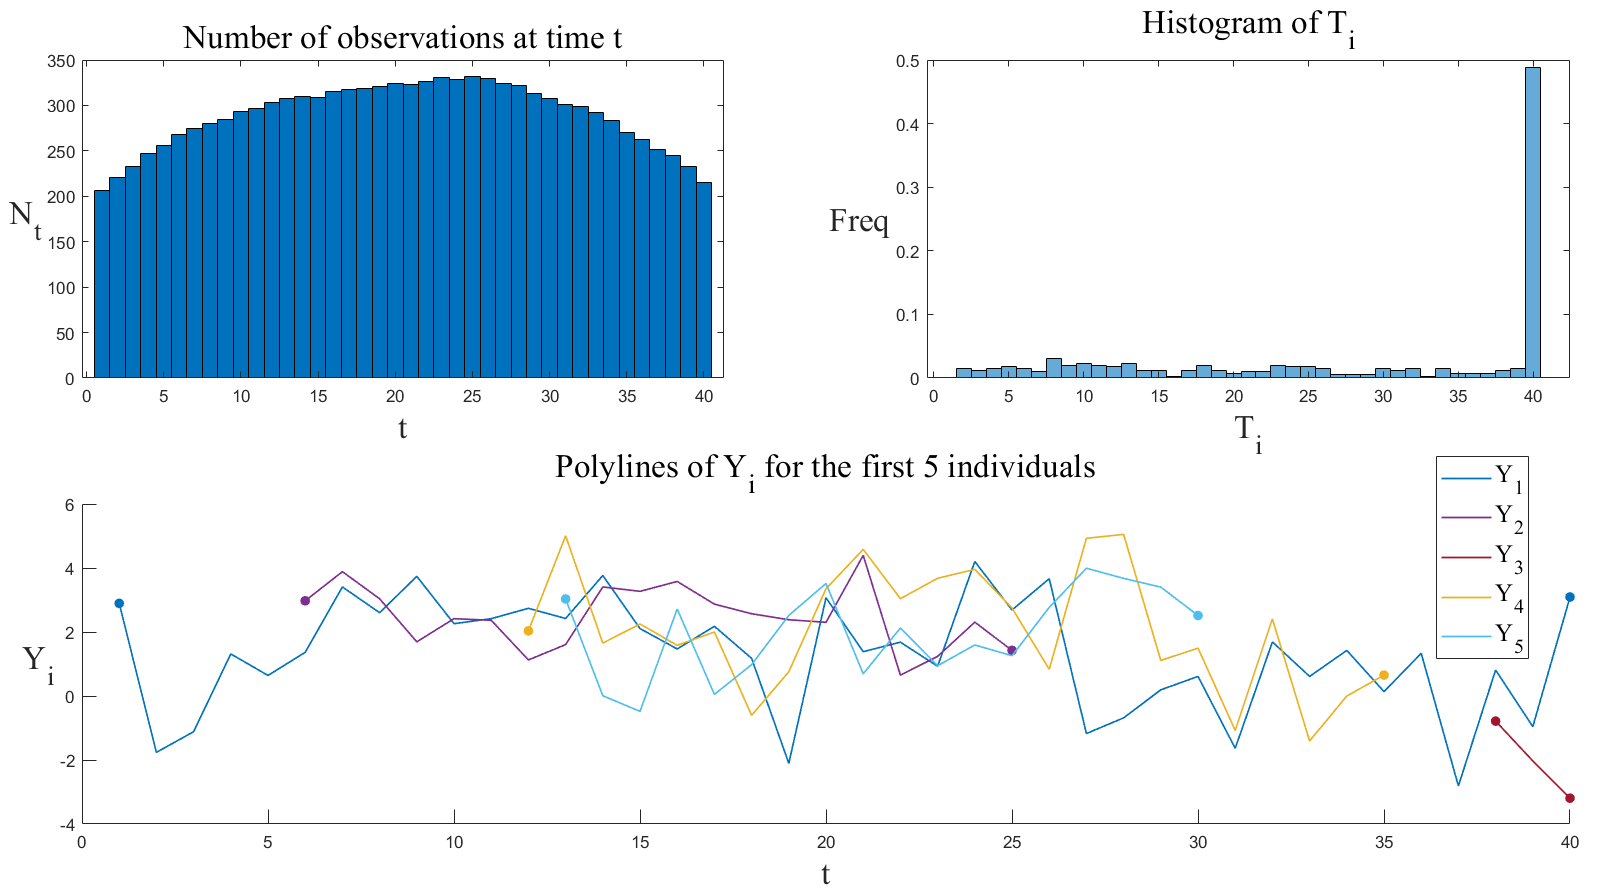
\includegraphics[width=0.85\textwidth]{pic/DGP.png}
    \caption{Characteristics of the unbalanced panel we generated}\label{pic_Yt}
\end{figure}
Figure~\ref{pic_Yt} illustrates 
key features of the simulated unbalanced dynamic network panel data with $N=400$, $T=40$ and $\mathrm{UP}=31.7\%$. It reveals that the number of observed nodes peaks during intermediate stages, with sparser observations in initial and terminal phases.
About 50\% of nodes are fully observed over the entire $T+1$ periods, while the remaining nodes have shorter observation windows, whose start times are drawn uniformly conditional on their durations.
%The figure shows that the number of observed nodes is more in the middle stage and less in the early and late stages. Almost half of the nodes have complete observations, while the observation duration distribution of the remaining nodes is relatively uniform.
\subsection{Simulation Results}

In the main simulation study, we investigate the finite-sample performance of the OWFE QMLE and its bias-corrected counterpart under varying configurations of $N \in \{100, 400, 1600\}$, $T \in \{10, 40\}$, and $\mathrm{UP}\in \{30\%, 60\%\}$. 
For the OWFE simulations, we consider two true parameter settings, $\theta_0=(0.5,0.2,0.1,1,1,1)$ and $\theta_0=(0.1,0.3,0.5,1,1,1)$, where $\theta_0=(\rho_0,\lambda_0,\nu_0,\gamma_0,\beta_0,\sigma^2_0)$. We also consider three error distributions: normal, centered exponential, and Laplace.
Under each setting, the estimation is repeated 1,000 times, and we evaluate the bias, standard deviation (SD), root mean square error (RMSE), and coverage probability (CP) of the estimators.

The OWFE simulation results are presented in Tables \ref{Tab_N130}-\ref{Tab_N160} and Tables D.1--D.6 in Supplementary Appendix D.1. 
Supplementary Appendix D.1 reports additional TWFE simulation results in Tables D.7--D.12 for \(\theta_0=(0.5,0.2,0.1,1,1,1)\) under the same error distributions and UP levels.
From the OWFE simulation tables, we obtain the following findings. 
\begin{enumerate}[(1)]
\item The biases of both the original estimator and the bias-corrected estimator decrease significantly as $T$ increases, but show little change as $N$ increases. Moreover, for fixed $N$ and $T$, a higher UP leads to larger bias. These findings are consistent with the theoretical bias of order $O_p(\frac{1}{c_u T})$.
\item Regardless of whether bias correction is applied, the standard deviations of most estimators are approximately halved when either $N$ or $T$ is quadrupled, consistent with the theoretical convergence rate of $1/\sqrt{n}$. An exception is $\hat{\gamma}$, whose standard deviation remains essentially unchanged as $T$ increases, aligning with the theoretical convergence rate of $1/\sqrt{c_uN}$.
Moreover, the standard deviation increases as the UP rises.
\item The original estimators exhibit substantial bias, especially for $\nu$ and $\sigma^2$, while the bias-corrected estimators significantly reduce the bias. The bias-corrected estimators show notable improvements in both bias and RMSE, and their CPs are also closer to the nominal levels of 95\% and 90\%. %In most cases where no improvement is observed, it is because the uncorrected estimators are already highly accurate, so randomness prevents the bias correction from yielding further gains.
\item As $N$ increases, there is a downward trend in CPs for both estimators, which is attributable to the asymptotic bias of order $O_p(\sqrt{N/T^3})$.
\end{enumerate}

The supplementary TWFE simulations in Tables D.7--D.12 display a similar pattern. The original TWFE estimator also exhibits noticeable finite-sample bias. After
bias correction, the biases and RMSEs are generally reduced, and the CPs move closer to the nominal levels. These results suggest that the proposed bias correction remains effective after introducing time fixed effects.


%When $N=1600$ and $T=10$, even after bias correction, both $\nu$ and $\sigma^2$ have low CP. This is because they have large inherent biases, and our asymptotic properties are derived as $T$ approaches infinity.

To examine the correctness of the asymptotic theory, we plot the kernel density curves of $\frac{\hat{\theta}_i-\theta_{0i}}{\mathrm{SE}_i}$, and $\frac{\hat{\theta}^1_i-\theta_{0i}}{\mathrm{SE}_i}$, where $\hat{\theta}_i$, $\hat{\theta}^1_i$ and $\theta_{0i}$ denote the $i$-th element of $\hat{\theta}$, $\hat{\theta}^1$ and $\theta_{0}$, respectively, and $\mathrm{SE}_i$ denotes the square root of the $i$-th diagonal element of $\frac{1}{n}\Sigma_{\theta_0,n}^{-1}(\Sigma_{\theta_0,n}+\Omega_{\theta_0,n})\Sigma_{\theta_0,n}^{-1}$.
These kernel densities are then compared with the probability density function (PDF) of the standard normal distribution. The results are shown in Figures \ref{Fig_N130}-\ref{Fig_N160} and Figures D.1-D.6 in Supplementary Appendix D.2. As illustrated in the figures, regardless of whether the estimators are bias corrected or not, their distributions become increasingly close to normality as the sample size increases. The bias-corrected estimators exhibit distributions that are closer to a centered normal distribution than the original ones.
%The tables show that as $N$ and $T$ increase, our estimators become increasingly precise. When $N$ or $T$ increases by a factor of four, the std of the estimators are roughly halved. This suggests that the convergence rate of our estimators is approximately $ O\left(\frac{1}{\sqrt{NT}}\right) $. Furthermore, the rmse exhibits a similar pattern to the std, except when $T$ is small for the estimations of $\nu$ and $\sigma^2$, where significant biases are observed. This indicates that when $T$ is small, our estimators might be biased, and therefore, bias correction is necessary when the sample size is limited. Our model performs similarly under different levels of $\mathrm{UP}$ because the data is not truly missing, but rather more ``sparse" in structure. Our method is capable of overcoming this sparsity and effectively modeling the data.
\begin{landscape}
\begin{table}[p]
\caption{Results of OWFE estimator with Normal error, UP=30\%, $\theta_0=(0.5,0.2,0.1,1,1,1)$.}
\label{Tab_N130}
\centering
\begin{threeparttable}
{
\resizebox{0.86\linewidth}{!}{
\begin{tabular}{ccrrrrrrccrrrrrr}
\hline
 &  & \multicolumn{1}{c}{$\rho$} & \multicolumn{1}{c}{$\lambda$} & \multicolumn{1}{c}{$\nu$} & \multicolumn{1}{c}{$\gamma$} & \multicolumn{1}{c}{$\beta$} & \multicolumn{1}{c}{$\sigma^2$} &  &  & \multicolumn{1}{c}{$\rho$} & \multicolumn{1}{c}{$\lambda$} & \multicolumn{1}{c}{$\nu$} & \multicolumn{1}{c}{$\gamma$} & \multicolumn{1}{c}{$\beta$} & \multicolumn{1}{c}{$\sigma^2$} \\ \hline
$T=10$ &  & \multicolumn{6}{c}{Before bias correction} & $T=40$ &  & \multicolumn{6}{c}{Before bias correction} \\ \cline{3-8} \cline{11-16} 
$N=100$ & BIAS & -0.0044 & 0.0327 & -0.0753 & -0.0348 & -0.0098 & -0.1594 & $N=100$ & BIAS & 0.0006 & 0.0077 & -0.0191 & -0.0014 & -0.0016 & -0.0399 \\
 & SD & 0.0268 & 0.0367 & 0.0299 & 0.1497 & 0.0427 & 0.0511 &  & SD & 0.0124 & 0.0178 & 0.0146 & 0.1426 & 0.0191 & 0.0275 \\
 & RMSE & 0.0271 & 0.0492 & 0.0810 & 0.1537 & 0.0438 & 0.1674 &  & RMSE & 0.0124 & 0.0194 & 0.0240 & 0.1426 & 0.0192 & 0.0484 \\
 & 95\%CP & 0.9340 & 0.8620 & 0.2810 & 0.9470 & 0.9370 & 0.1530 &  & 95\%CP & 0.9550 & 0.9190 & 0.7070 & 0.9510 & 0.9570 & 0.6860 \\
 & 90\%CP & 0.8640 & 0.7660 & 0.1920 & 0.8900 & 0.8890 & 0.0930 &  & 90\%CP & 0.8910 & 0.8740 & 0.6080 & 0.8970 & 0.9060 & 0.5630 \\ \cline{2-8} \cline{10-16} 
 &  & \multicolumn{6}{c}{After bias correction} &  &  & \multicolumn{6}{c}{After bias correction} \\ \cline{3-8} \cline{11-16} 
 & BIAS & \textbf{-0.0034} & \textbf{0.0061} & \textbf{-0.0159} & \textbf{-0.0064} & \textbf{-0.0005} & \textbf{-0.0397} &  & BIAS & \textbf{0.0002} & \textbf{0.0001} & \textbf{-0.0010} & 0.0019 & \textbf{-0.0007} & \textbf{-0.0053} \\
 & SD & \textbf{0.0267} & 0.0375 & 0.0311 & \textbf{0.1495} & \textbf{0.0426} & 0.0580 &  & SD & 0.0124 & 0.0180 & 0.0148 & \textbf{0.1425} & 0.0191 & 0.0284 \\
 & RMSE & \textbf{0.0269} & \textbf{0.0380} & \textbf{0.0349} & \textbf{0.1497} & \textbf{0.0426} & \textbf{0.0703} &  & RMSE & \textbf{0.0124} & \textbf{0.0180} & \textbf{0.0149} & \textbf{0.1425} & \textbf{0.0191} & \textbf{0.0289} \\
 & 95\%CP & \textbf{0.9360} & \textbf{0.9380} & \textbf{0.9100} & \textit{0.9470} & \textbf{0.9410} & \textbf{0.8770} &  & 95\%CP & \textit{0.9550} & \textbf{0.9490} & \textbf{0.9430} & 0.9530 & \textbf{0.9560} & \textbf{0.9420} \\
 & 90\%CP & \textbf{0.8670} & \textbf{0.9000} & \textbf{0.8380} & \textbf{0.8990} & \textbf{0.8920} & \textbf{0.7780} &  & 90\%CP & 0.8890 & \textbf{0.8950} & \textbf{0.8820} & 0.8960 & \textbf{0.9020} & \textbf{0.8900} \\ \hline
$T=10$ &  & \multicolumn{6}{c}{Before bias correction} & $T=40$ &  & \multicolumn{6}{c}{Before bias correction} \\ \cline{3-8} \cline{11-16} 
$N=400$ & BIAS & -0.0021 & 0.0339 & -0.0748 & -0.0341 & -0.0126 & -0.1525 & $N=400$ & BIAS & 0.0000 & 0.0082 & -0.0194 & -0.0027 & 0.0001 & -0.0364 \\
 & SD & 0.0136 & 0.0189 & 0.0146 & 0.0765 & 0.0207 & 0.0259 &  & SD & 0.0063 & 0.0090 & 0.0070 & 0.0705 & 0.0098 & 0.0142 \\
 & RMSE & 0.0137 & 0.0388 & 0.0762 & 0.0838 & 0.0242 & 0.1546 &  & RMSE & 0.0063 & 0.0122 & 0.0206 & 0.0706 & 0.0098 & 0.0391 \\
 & 95\%CP & 0.9360 & 0.5630 & 0.0010 & 0.9080 & 0.9070 & 0.0000 &  & 95\%CP & 0.9540 & 0.8640 & 0.2120 & 0.9590 & 0.9500 & 0.2440 \\
 & 90\%CP & 0.8730 & 0.4490 & 0.0000 & 0.8450 & 0.8370 & 0.0000 &  & 90\%CP & 0.9080 & 0.7630 & 0.1390 & 0.9020 & 0.8930 & 0.1700 \\ \cline{2-8} \cline{10-16} 
 &  & \multicolumn{6}{c}{After bias correction} &  &  & \multicolumn{6}{c}{After bias correction} \\ \cline{3-8} \cline{11-16} 
 & BIAS & \textbf{-0.0012} & \textbf{0.0064} & \textbf{-0.0152} & \textbf{-0.0065} & \textbf{-0.0033} & \textbf{-0.0319} &  & BIAS & -0.0004 & \textbf{0.0006} & \textbf{-0.0013} & \textbf{0.0004} & 0.0010 & \textbf{-0.0017} \\
 & SD & 0.0136 & 0.0194 & 0.0151 & 0.0768 & \textbf{0.0206} & 0.0294 &  & SD & 0.0063 & 0.0091 & 0.0071 & 0.0707 & \textbf{0.0098} & 0.0146 \\
 & RMSE & \textbf{0.0136} & \textbf{0.0204} & \textbf{0.0214} & \textbf{0.0771} & \textbf{0.0208} & \textbf{0.0434} &  & RMSE & 0.0063 & \textbf{0.0091} & \textbf{0.0072} & 0.0707 & 0.0099 & \textbf{0.0147} \\
 & 95\%CP & 0.9330 & \textbf{0.9350} & \textbf{0.8290} & \textbf{0.9260} & \textbf{0.9540} & \textbf{0.7590} &  & 95\%CP & \textbf{0.9500} & \textbf{0.9460} & \textbf{0.9420} & \textit{0.9590} & 0.9450 & \textbf{0.9310} \\
 & 90\%CP & \textbf{0.8750} & \textbf{0.8670} & \textbf{0.7260} & \textbf{0.8730} & \textbf{0.9000} & \textbf{0.6690} &  & 90\%CP & \textbf{0.9020} & \textbf{0.9040} & \textbf{0.8830} & \textbf{0.9010} & \textbf{0.9010} & \textbf{0.8670} \\ \hline
$T=10$ &  & \multicolumn{6}{c}{Before bias correction} & $T=40$ &  & \multicolumn{6}{c}{Before bias correction} \\ \cline{3-8} \cline{11-16} 
$N=1600$ & BIAS & -0.0020 & 0.0338 & -0.0748 & -0.0343 & -0.0114 & -0.1530 & $N=1600$ & BIAS & 0.0004 & 0.0078 & -0.0192 & -0.0033 & -0.0011 & -0.0371 \\
 & SD & 0.0071 & 0.0090 & 0.0075 & 0.0357 & 0.0102 & 0.0127 &  & SD & 0.0032 & 0.0047 & 0.0034 & 0.0352 & 0.0048 & 0.0067 \\
 & RMSE & 0.0073 & 0.0350 & 0.0751 & 0.0496 & 0.0153 & 0.1535 &  & RMSE & 0.0032 & 0.0090 & 0.0195 & 0.0354 & 0.0049 & 0.0377 \\
 & 95\%CP & 0.9300 & 0.0480 & 0.0000 & 0.8550 & 0.8100 & 0.0000 &  & 95\%CP & 0.9530 & 0.6140 & 0.0010 & 0.9500 & 0.9520 & 0.0010 \\
 & 90\%CP & 0.8630 & 0.0210 & 0.0000 & 0.7690 & 0.6980 & 0.0000 &  & 90\%CP & 0.9020 & 0.4960 & 0.0010 & 0.8970 & 0.8920 & 0.0000 \\ \cline{2-8} \cline{10-16} 
 &  & \multicolumn{6}{c}{After bias correction} &  &  & \multicolumn{6}{c}{After bias correction} \\ \cline{3-8} \cline{11-16} 
 & BIAS & \textbf{-0.0011} & \textbf{0.0062} & \textbf{-0.0152} & \textbf{-0.0067} & \textbf{-0.0022} & \textbf{-0.0325} &  & BIAS & \textbf{0.0000} & \textbf{0.0002} & \textbf{-0.0011} & \textbf{-0.0001} & \textbf{-0.0002} & \textbf{-0.0025} \\
 & SD & 0.0071 & 0.0094 & 0.0078 & 0.0359 & \textbf{0.0102} & 0.0144 &  & SD & 0.0032 & 0.0047 & 0.0034 & 0.0352 & \textbf{0.0048} & 0.0069 \\
 & RMSE & \textbf{0.0072} & \textbf{0.0112} & \textbf{0.0171} & \textbf{0.0365} & \textbf{0.0104} & \textbf{0.0355} &  & RMSE & \textbf{0.0032} & \textbf{0.0047} & \textbf{0.0036} & \textbf{0.0352} & \textbf{0.0048} & \textbf{0.0073} \\
 & 95\%CP & \textbf{0.9310} & \textbf{0.9000} & \textbf{0.4840} & \textbf{0.9530} & \textbf{0.9450} & \textbf{0.3380} &  & 95\%CP & 0.9580 & \textbf{0.9450} & \textbf{0.9450} & 0.9490 & 0.9580 & \textbf{0.9360} \\
 & 90\%CP & \textbf{0.8720} & \textbf{0.8330} & \textbf{0.3690} & \textbf{0.9040} & \textbf{0.9060} & \textbf{0.2280} &  & 90\%CP & \textbf{0.9000} & \textbf{0.8900} & \textbf{0.8830} & 0.8960 & \textbf{0.9070} & \textbf{0.8790} \\ \hline
\end{tabular}}}
\par\smallskip
\begin{minipage}[t]{0.86\linewidth}
\footnotesize
Notes: $\mathrm{UP}=1-\frac{n}{NT}$. In the table, \textbf{bold} numbers indicate that the bias-corrected results have improved, while \textit{italicized} numbers indicate that the bias-corrected results perform equally well as before. 
The 95\%CP and 90\%CP  indicate the frequencies that the true parameter value is contained within the 95\% and 90\% confidence intervals of the estimator, respectively.
\end{minipage}
\end{threeparttable}
\end{table}
\end{landscape}

\begin{landscape}
\begin{table}[p]
\caption{Results of OWFE estimator with Normal error, UP=60\%, $\theta_0=(0.5,0.2,0.1,1,1,1)$.}
\label{Tab_N160}
\centering
\begin{threeparttable}
{
\resizebox{0.86\linewidth}{!}{
\begin{tabular}{ccrrrrrrccrrrrrr}
\hline
 &  & \multicolumn{1}{c}{$\rho$} & \multicolumn{1}{c}{$\lambda$} & \multicolumn{1}{c}{$\nu$} & \multicolumn{1}{c}{$\gamma$} & \multicolumn{1}{c}{$\beta$} & \multicolumn{1}{c}{$\sigma^2$} &  &  & \multicolumn{1}{c}{$\rho$} & \multicolumn{1}{c}{$\lambda$} & \multicolumn{1}{c}{$\nu$} & \multicolumn{1}{c}{$\gamma$} & \multicolumn{1}{c}{$\beta$} & \multicolumn{1}{c}{$\sigma^2$} \\ \hline
$T=10$ &  & \multicolumn{6}{c}{Before bias correction} & $T=40$ &  & \multicolumn{6}{c}{Before bias correction} \\ \cline{3-8} \cline{11-16} 
$N=100$ & BIAS & -0.0093 & 0.0605 & -0.1358 & -0.0929 & -0.0337 & -0.2862 & $N=100$ & BIAS & 0.0004 & 0.0141 & -0.0321 & -0.0147 & -0.0029 & -0.0694 \\
 & SD & 0.0307 & 0.0468 & 0.0440 & 0.1348 & 0.0613 & 0.0613 &  & SD & 0.0141 & 0.0203 & 0.0185 & 0.1098 & 0.0263 & 0.0352 \\
 & RMSE & 0.0321 & 0.0765 & 0.1428 & 0.1638 & 0.0700 & 0.2927 &  & RMSE & 0.0141 & 0.0247 & 0.0370 & 0.1108 & 0.0264 & 0.0778 \\
 & 95\%CP & 0.9100 & 0.7650 & 0.1200 & 0.8810 & 0.9000 & 0.0100 &  & 95\%CP & 0.9470 & 0.9070 & 0.6060 & 0.9570 & 0.9410 & 0.5100 \\
 & 90\%CP & 0.8370 & 0.6700 & 0.0670 & 0.8260 & 0.8310 & 0.0020 &  & 90\%CP & 0.8870 & 0.8320 & 0.4840 & 0.9040 & 0.8990 & 0.3840 \\ \cline{2-8} \cline{10-16} 
 &  & \multicolumn{6}{c}{After bias correction} &  &  & \multicolumn{6}{c}{After bias correction} \\ \cline{3-8} \cline{11-16} 
 & BIAS & \textbf{-0.0062} & \textbf{0.0212} & \textbf{-0.0481} & \textbf{-0.0345} & \textbf{-0.0112} & \textbf{-0.1083} &  & BIAS & \textbf{0.0000} & \textbf{0.0006} & \textbf{-0.0031} & \textbf{-0.0074} & \textbf{-0.0006} & \textbf{-0.0105} \\
 & SD & \textbf{0.0308} & 0.0484 & 0.0458 & \textbf{0.1341} & \textbf{0.0612} & 0.0744 &  & SD & 0.0141 & 0.0206 & 0.0188 & 0.1099 & \textbf{0.0262} & 0.0371 \\
 & RMSE & \textbf{0.0314} & \textbf{0.0528} & \textbf{0.0664} & \textbf{0.1385} & \textbf{0.0623} & \textbf{0.1314} &  & RMSE & 0.0141 & \textbf{0.0206} & \textbf{0.0191} & \textbf{0.1102} & \textbf{0.0262} & \textbf{0.0386} \\
 & 95\%CP & \textbf{0.9200} & \textbf{0.9180} & \textbf{0.7850} & \textbf{0.9380} & \textbf{0.9430} & \textbf{0.6750} &  & 95\%CP & 0.9460 & \textbf{0.9490} & \textbf{0.9500} & 0.9590 & \textbf{0.9460} & \textbf{0.9310} \\
 & 90\%CP & \textbf{0.8490} & \textbf{0.8530} & \textbf{0.6910} & \textbf{0.8710} & \textbf{0.8740} & \textbf{0.5500} &  & 90\%CP & \textbf{0.8880} & \textbf{0.9170} & \textbf{0.8890} & 0.9090 & 0.9030 & \textbf{0.8840} \\ \hline
$T=10$ &  & \multicolumn{6}{c}{Before bias correction} & $T=40$ &  & \multicolumn{6}{c}{Before bias correction} \\ \cline{3-8} \cline{11-16} 
$N=400$ & BIAS & -0.0061 & 0.0583 & -0.1302 & -0.0861 & -0.0316 & -0.2766 & $N=400$ & BIAS & 0.0003 & 0.0145 & -0.0317 & -0.0069 & -0.0026 & -0.0660 \\
 & SD & 0.0153 & 0.0225 & 0.0215 & 0.0645 & 0.0300 & 0.0311 &  & SD & 0.0068 & 0.0101 & 0.0094 & 0.0573 & 0.0129 & 0.0177 \\
 & RMSE & 0.0165 & 0.0625 & 0.1320 & 0.1076 & 0.0435 & 0.2784 &  & RMSE & 0.0068 & 0.0176 & 0.0331 & 0.0577 & 0.0131 & 0.0683 \\
 & 95\%CP & 0.9050 & 0.2960 & 0.0000 & 0.7510 & 0.8230 & 0.0000 &  & 95\%CP & 0.9470 & 0.7290 & 0.0810 & 0.9430 & 0.9450 & 0.0410 \\
 & 90\%CP & 0.8260 & 0.1980 & 0.0000 & 0.6390 & 0.7240 & 0.0000 &  & 90\%CP & 0.8990 & 0.6200 & 0.0390 & 0.8840 & 0.9120 & 0.0220 \\ \cline{2-8} \cline{10-16} 
 &  & \multicolumn{6}{c}{After bias correction} &  &  & \multicolumn{6}{c}{After bias correction} \\ \cline{3-8} \cline{11-16} 
 & BIAS & \textbf{-0.0032} & \textbf{0.0179} & \textbf{-0.0426} & \textbf{-0.0282} & \textbf{-0.0095} & \textbf{-0.0963} &  & BIAS & \textbf{-0.0001} & \textbf{0.0009} & \textbf{-0.0028} & \textbf{0.0004} & \textbf{-0.0003} & \textbf{-0.0071} \\
 & SD & \textbf{0.0152} & 0.0232 & 0.0221 & \textbf{0.0635} & \textbf{0.0299} & 0.0378 &  & SD & 0.0068 & 0.0103 & 0.0096 & 0.0570 & 0.0129 & 0.0187 \\
 & RMSE & \textbf{0.0156} & \textbf{0.0293} & \textbf{0.0479} & \textbf{0.0695} & \textbf{0.0313} & \textbf{0.1035} &  & RMSE & 0.0068 & \textbf{0.0103} & \textbf{0.0100} & \textbf{0.0570} & \textbf{0.0129} & \textbf{0.0200} \\
 & 95\%CP & \textbf{0.9230} & \textbf{0.8910} & \textbf{0.4940} & \textbf{0.9320} & \textbf{0.9360} & \textbf{0.2560} &  & 95\%CP & \textit{0.9470} & \textbf{0.9470} & \textbf{0.9320} & 0.9390 & \textbf{0.9510} & \textbf{0.9250} \\
 & 90\%CP & \textbf{0.8560} & \textbf{0.8090} & \textbf{0.3820} & \textbf{0.8830} & \textbf{0.8850} & \textbf{0.1660} &  & 90\%CP & 0.8940 & \textbf{0.9000} & \textbf{0.8740} & \textbf{0.8980} & \textbf{0.9110} & \textbf{0.8710} \\ \hline
$T=10$ &  & \multicolumn{6}{c}{Before bias correction} & $T=40$ &  & \multicolumn{6}{c}{Before bias correction} \\ \cline{3-8} \cline{11-16} 
$N=1600$ & BIAS & -0.0055 & 0.0591 & -0.1305 & -0.0868 & -0.0329 & -0.2748 & $N=1600$ & BIAS & 0.0003 & 0.0147 & -0.0319 & -0.0083 & -0.0025 & -0.0653 \\
 & SD & 0.0077 & 0.0118 & 0.0108 & 0.0322 & 0.0152 & 0.0155 &  & SD & 0.0035 & 0.0050 & 0.0047 & 0.0268 & 0.0066 & 0.0091 \\
 & RMSE & 0.0095 & 0.0602 & 0.1310 & 0.0926 & 0.0363 & 0.2752 &  & RMSE & 0.0035 & 0.0155 & 0.0323 & 0.0281 & 0.0070 & 0.0659 \\
 & 95\%CP & 0.8560 & 0.0020 & 0.0000 & 0.2400 & 0.4000 & 0.0000 &  & 95\%CP & 0.9500 & 0.1890 & 0.0000 & 0.9500 & 0.9380 & 0.0000 \\
 & 90\%CP & 0.7740 & 0.0010 & 0.0000 & 0.1650 & 0.2880 & 0.0000 &  & 90\%CP & 0.8980 & 0.1120 & 0.0000 & 0.8970 & 0.8770 & 0.0000 \\ \cline{2-8} \cline{10-16} 
 &  & \multicolumn{6}{c}{After bias correction} &  &  & \multicolumn{6}{c}{After bias correction} \\ \cline{3-8} \cline{11-16} 
 & BIAS & \textbf{-0.0028} & \textbf{0.0185} & \textbf{-0.0427} & \textbf{-0.0287} & \textbf{-0.0109} & \textbf{-0.0940} &  & BIAS & \textbf{-0.0002} & \textbf{0.0011} & \textbf{-0.0031} & \textbf{-0.0010} & \textbf{-0.0003} & \textbf{-0.0064} \\
 & SD & \textbf{0.0076} & 0.0122 & 0.0114 & \textbf{0.0320} & \textbf{0.0151} & 0.0187 &  & SD & \textbf{0.0035} & 0.0051 & 0.0048 & 0.0269 & 0.0066 & 0.0096 \\
 & RMSE & \textbf{0.0081} & \textbf{0.0222} & \textbf{0.0442} & \textbf{0.0430} & \textbf{0.0186} & \textbf{0.0959} &  & RMSE & \textbf{0.0035} & \textbf{0.0052} & \textbf{0.0057} & \textbf{0.0269} & \textbf{0.0066} & \textbf{0.0115} \\
 & 95\%CP & \textbf{0.9020} & \textbf{0.6440} & \textbf{0.0230} & \textbf{0.8600} & \textbf{0.8880} & \textit{0.0000} &  & 95\%CP & 0.9480 & \textbf{0.9540} & \textbf{0.8960} & 0.9710 & \textbf{0.9520} & \textbf{0.8850} \\
 & 90\%CP & \textbf{0.8490} & \textbf{0.5270} & \textbf{0.0100} & \textbf{0.7800} & \textbf{0.7980} & \textit{0.0000} &  & 90\%CP & 0.8970 & \textbf{0.9090} & \textbf{0.8180} & 0.9070 & \textbf{0.9080} & \textbf{0.7870} \\ \hline
\end{tabular}
}}
\par\smallskip
\begin{minipage}[t]{0.86\linewidth}
\footnotesize
Notes: $\mathrm{UP}=1-\frac{n}{NT}$. In the table, \textbf{bold} numbers indicate that the bias-corrected results have improved, while \textit{italicized} numbers indicate that the bias-corrected results perform equally well as before. 
The 95\%CP and 90\%CP  indicate the frequencies that the true parameter value is contained within the 95\% and 90\% confidence intervals of the estimator, respectively.
\end{minipage}
\end{threeparttable}
\end{table}
\end{landscape}


\begin{figure}[h]
\centering
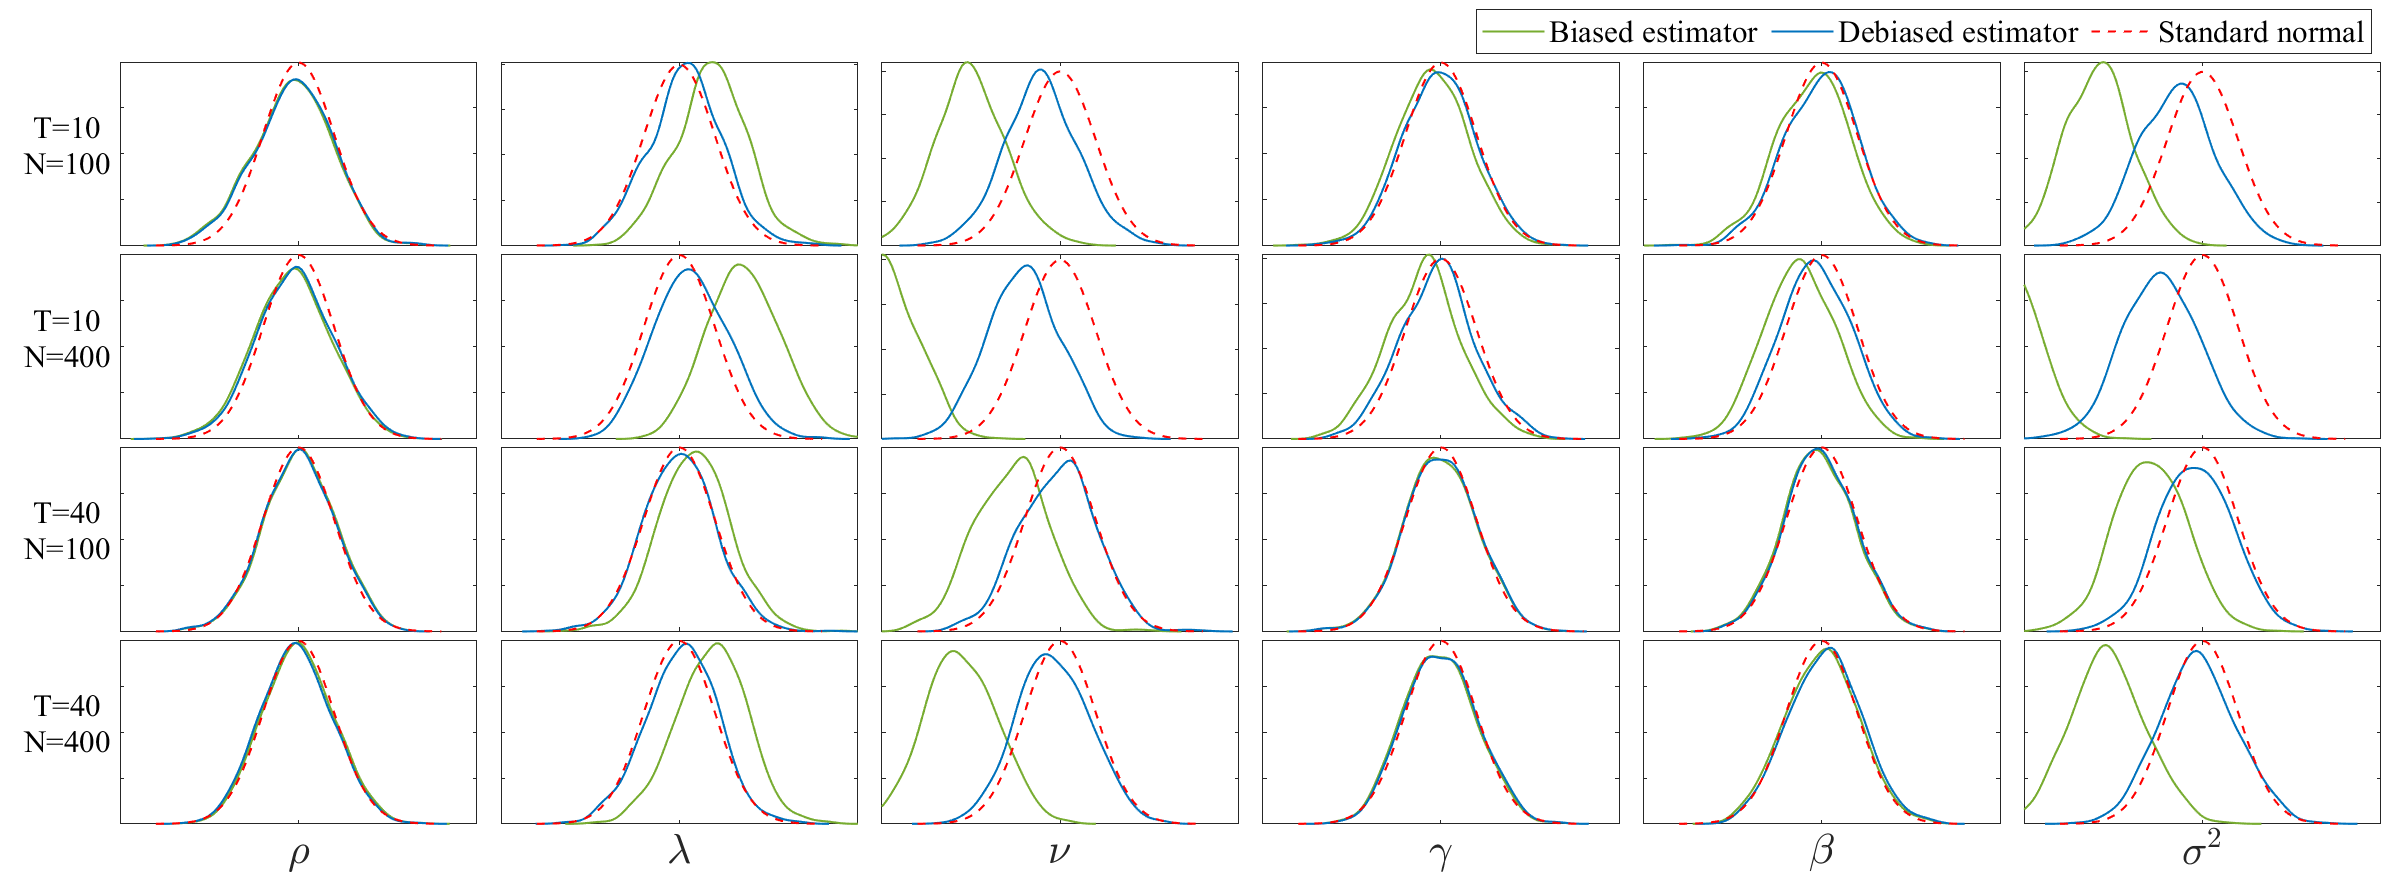
\includegraphics[width=\textwidth]{pic/N130.png}
\caption{PDF of OWFE standardized estimator with normal error, UP=30\%.}
\label{Fig_N130}
\end{figure}

\begin{figure}[h]
\centering
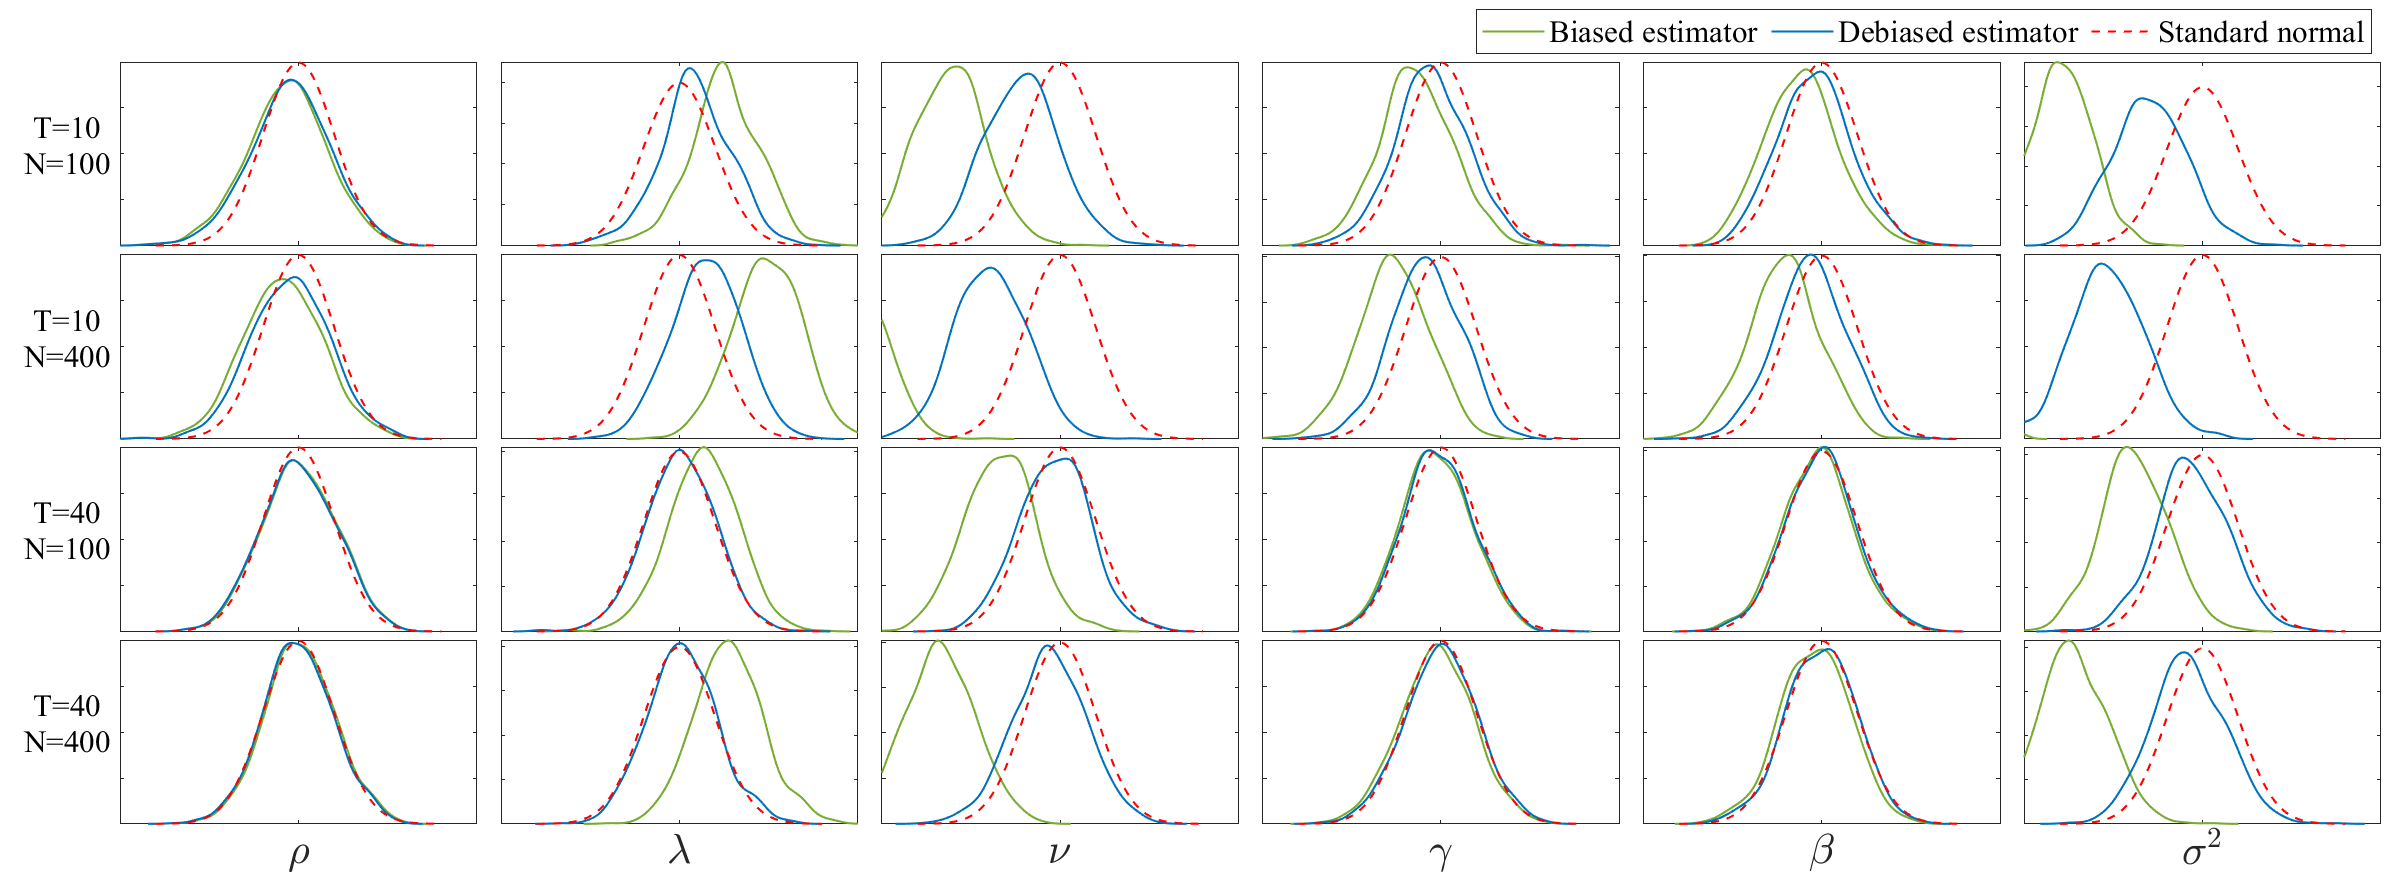
\includegraphics[width=\textwidth]{pic/N160.png}
\caption{PDF of OWFE standardized estimator with normal error, UP=60\%.}
\label{Fig_N160}
\end{figure}

\section{Real Data Analysis}\label{section5}

To assess our model's ability to capture the dynamics of unbalanced spatio-temporal panel data, we take the short-term rental market as the empirical application. In recent years, Airbnb, as a leading global platform for short-term accommodation, has expanded rapidly across cities and regions, and its supply and pricing dynamics have attracted extensive academic attention. 
More importantly, Airbnb data naturally exhibit an unbalanced panel structure: the set of available listings is not identical across time periods, and many listings are not observed throughout the entire sample period. This provides a representative and complex empirical setting for our study.
A large body of literature has already examined the rental pricing of Airbnb properties, such as the studies by \cite{su9091635}, \cite{GYODI2021104319}, and \cite{WANG2023100743}, which apply spatial econometric methods to cross-sectional data of Airbnb listings.
\cite{Juan2021} employ an unbalanced dynamic panel data model to analyze the impact of Airbnb listings on the Spanish tourism markets. Their model does not account for the spatial dependence in the data.
\cite{GUNTER2020104000} use a static spatial panel model to explore the substitution or complementarity relationship between Airbnb and traditional accommodations. However, their analysis is restricted to a balanced subsample of listings that are continuously observed over a long period, which accounts for less than $10\%$ of the total sample. This balanced spatial panel model neglects the spatial spillover effects from short-lived listings and does not account for the temporal dynamics in rental prices. While there have been studies using various models to analyze Airbnb rental prices, none simultaneously account for spatial spillover effects, temporal dynamics (e.g., price lags), and the unbalanced nature of the panel data. This is precisely what our model is designed to achieve.

We collect monthly Airbnb listing data from Inside Airbnb for two regions: New Zealand and New York City\footnote{\url{https://insideairbnb.com}}. The New Zealand raw data contain 31 monthly snapshots from May 13, 2023 to November 7, 2025, and the New York City raw data contain 18 monthly snapshots from June 4, 2024 to November 1, 2025. Each listing includes information such as rental price, geographic coordinates, availability over the next 30 days, and other listing-level characteristics.

To examine how short-term rental market dynamics vary across areas and spatial scales, we focus on six local markets. In New Zealand, the three samples are ward-level local markets: Waitemat\={a} and Gulf Ward, Queenstown-Wakatipu Ward, and Pukeh\={i}nau/Lambton Ward. For readability, we refer to them as Auckland, Queenstown, and Wellington, respectively, in the tables. In New York City, the three samples are the neighborhoods of Williamsburg, Midtown, and Hell's Kitchen. Within each local market, the dependent variable is the logarithm of rental price.

The empirical analysis uses the TWFE extension developed in Section~\ref{sec:twoway_extension}. The covariates in the empirical specification are the listing's own availability over the next 30 days, denoted by avail30d, and a neighborhood-level availability measure, denoted by avgAvail30d1km.

The unbalanced panel for Auckland, i.e., Waitemat\={a} and Gulf Ward, is visualized in Figure~\ref{pic_NewZealand_NT}. This sample contains $N=5{,}896$ listings, $T=30$ monthly periods, and $n=80{,}716$ observations, with an unbalancedness proportion of $\mathrm{UP}=54.37\%$. The corresponding sample sizes and unbalancedness proportions for the other local markets are reported in Tables~\ref{Tab_Comv_TWFE} and \ref{Tab_ComV_TWFE}. The descriptive statistics of all six datasets are reported in Supplementary Appendix E, Table E.1.

\begin{figure}[h]
    \centering
    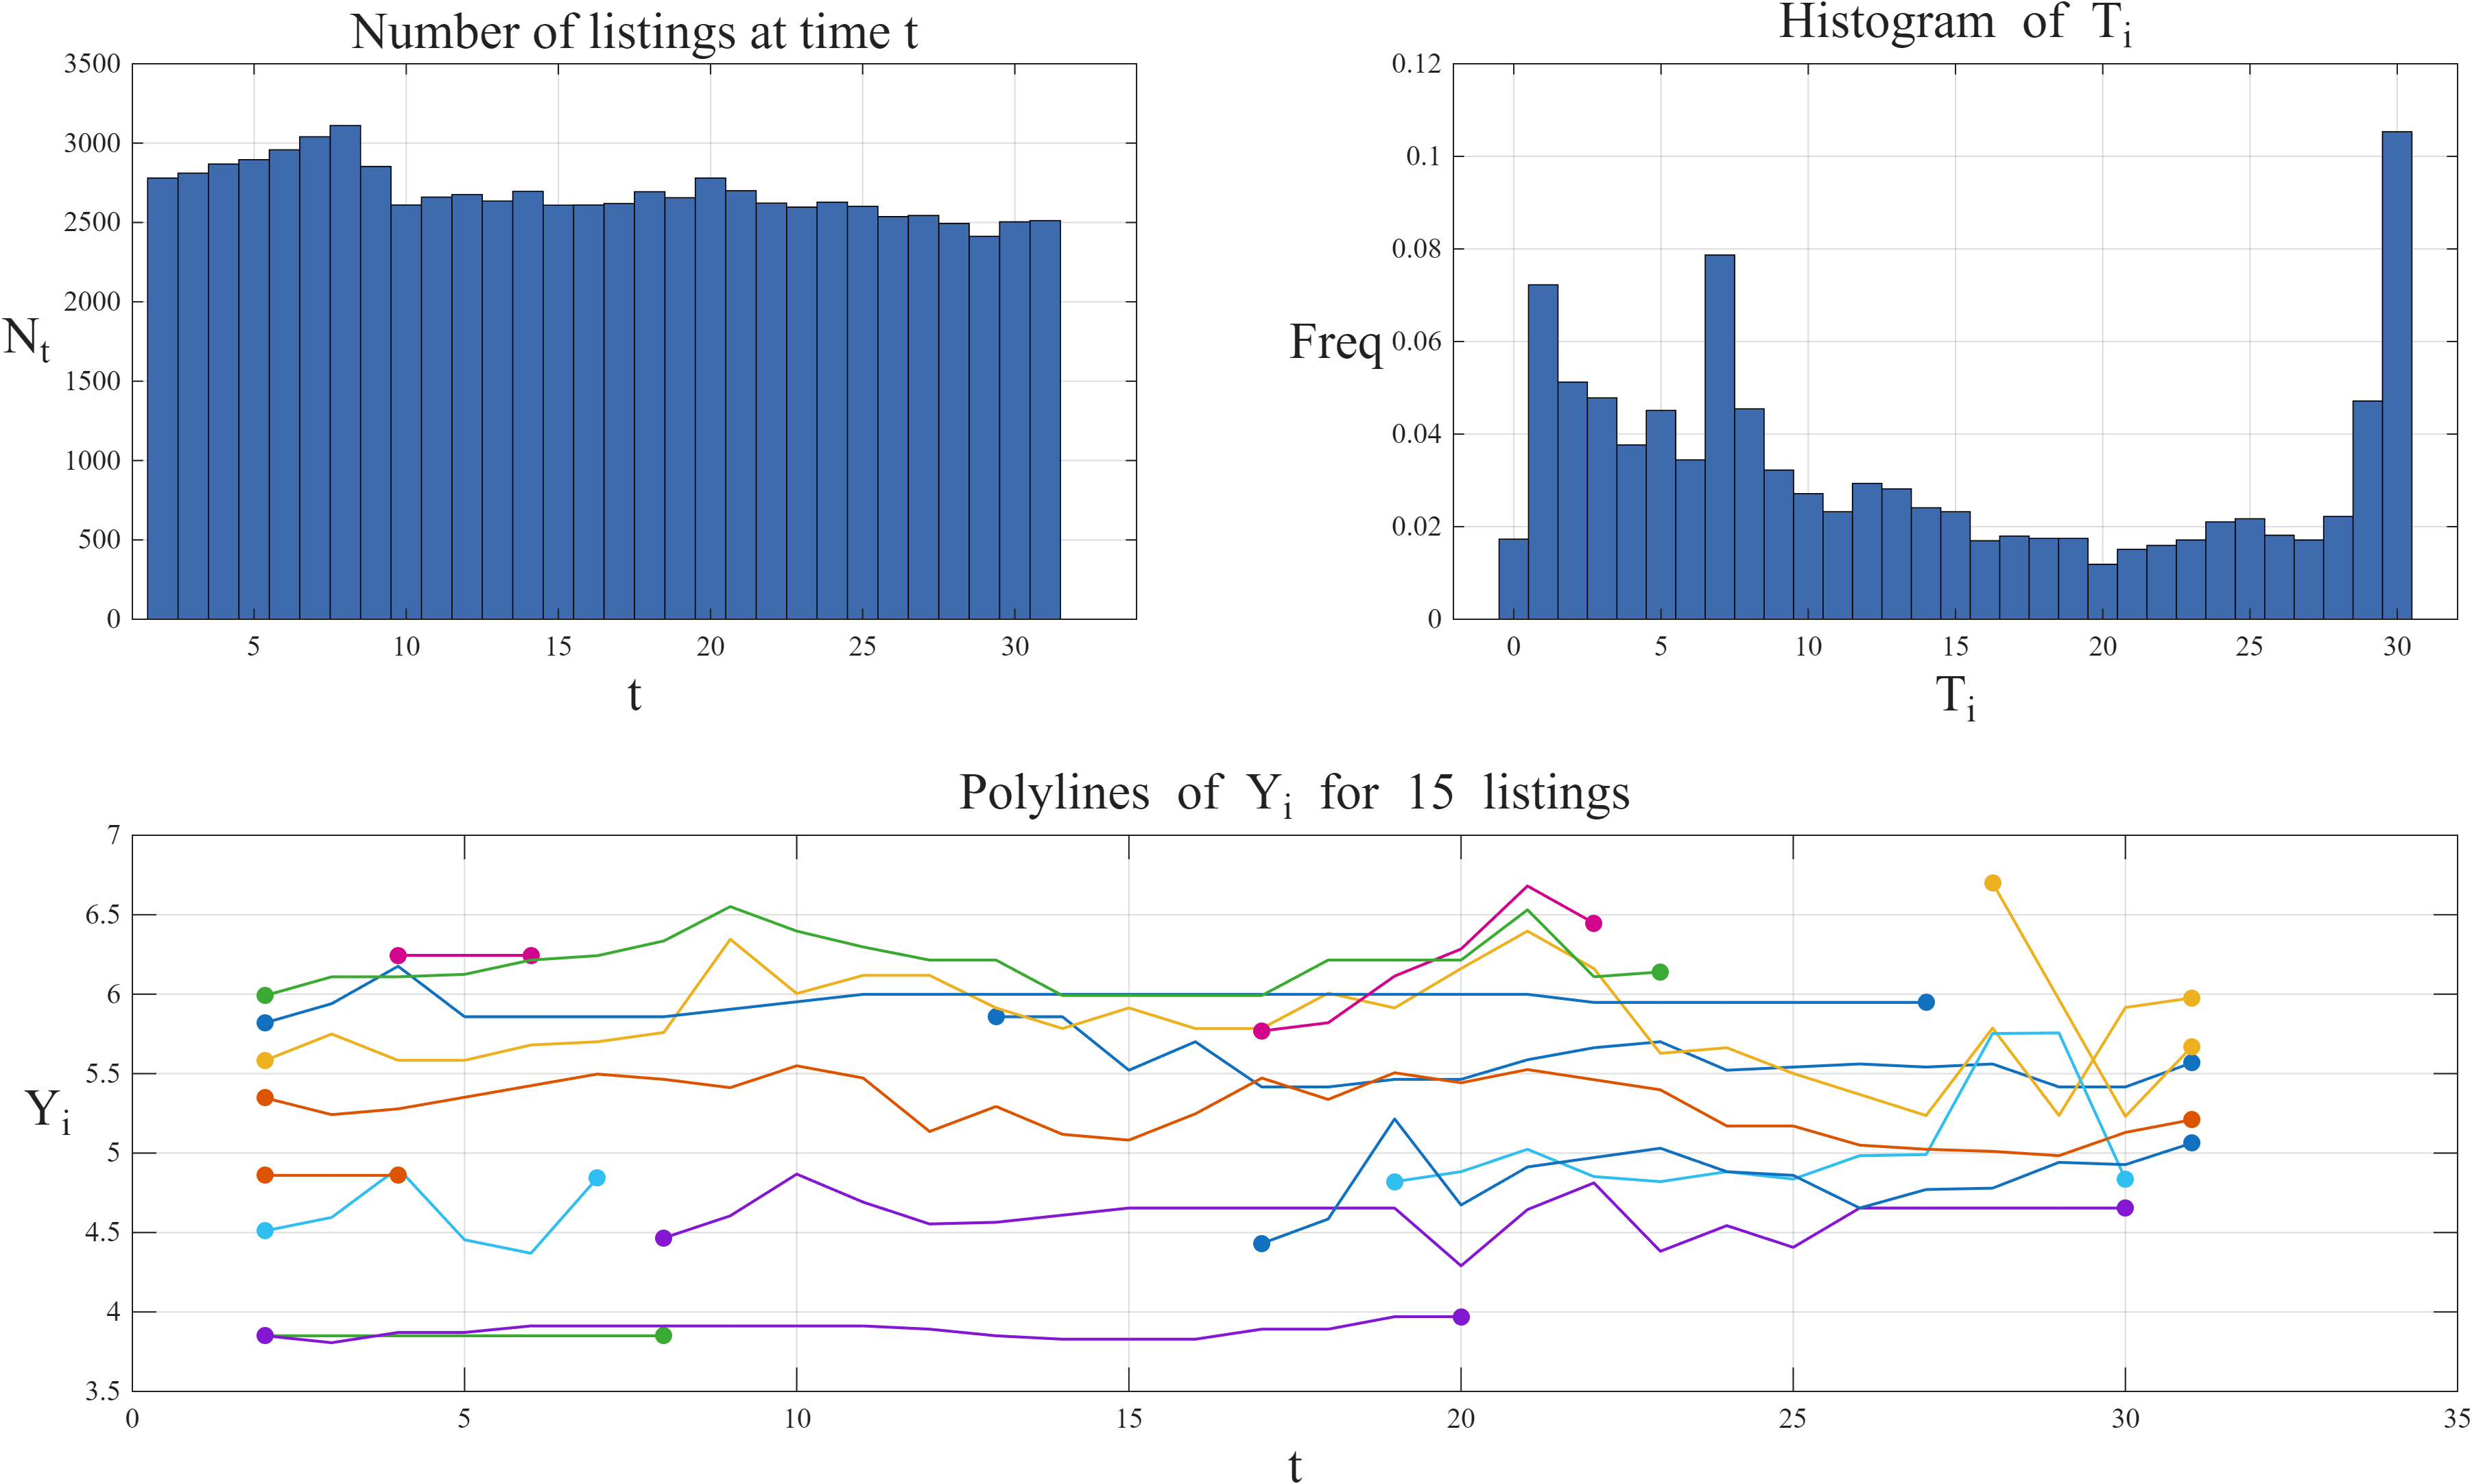
\includegraphics[width=\linewidth]{pic/NZ_NT.png}
    \caption{Characteristics of the unbalanced panel of the listing data in Auckland}
    \label{pic_NewZealand_NT}
\end{figure}

Figures~\ref{pic_geosc_MT} and~\ref{pic_geosc_QT} display the geographical distribution of log rental prices for listings in Midtown and Queenstown, respectively. The color shading corresponds to the magnitude of log rental price, with darker tones indicating lower values. These figures show that the log rental prices exhibit obvious spatial and temporal correlation.

\begin{figure}[h]
    \centering
    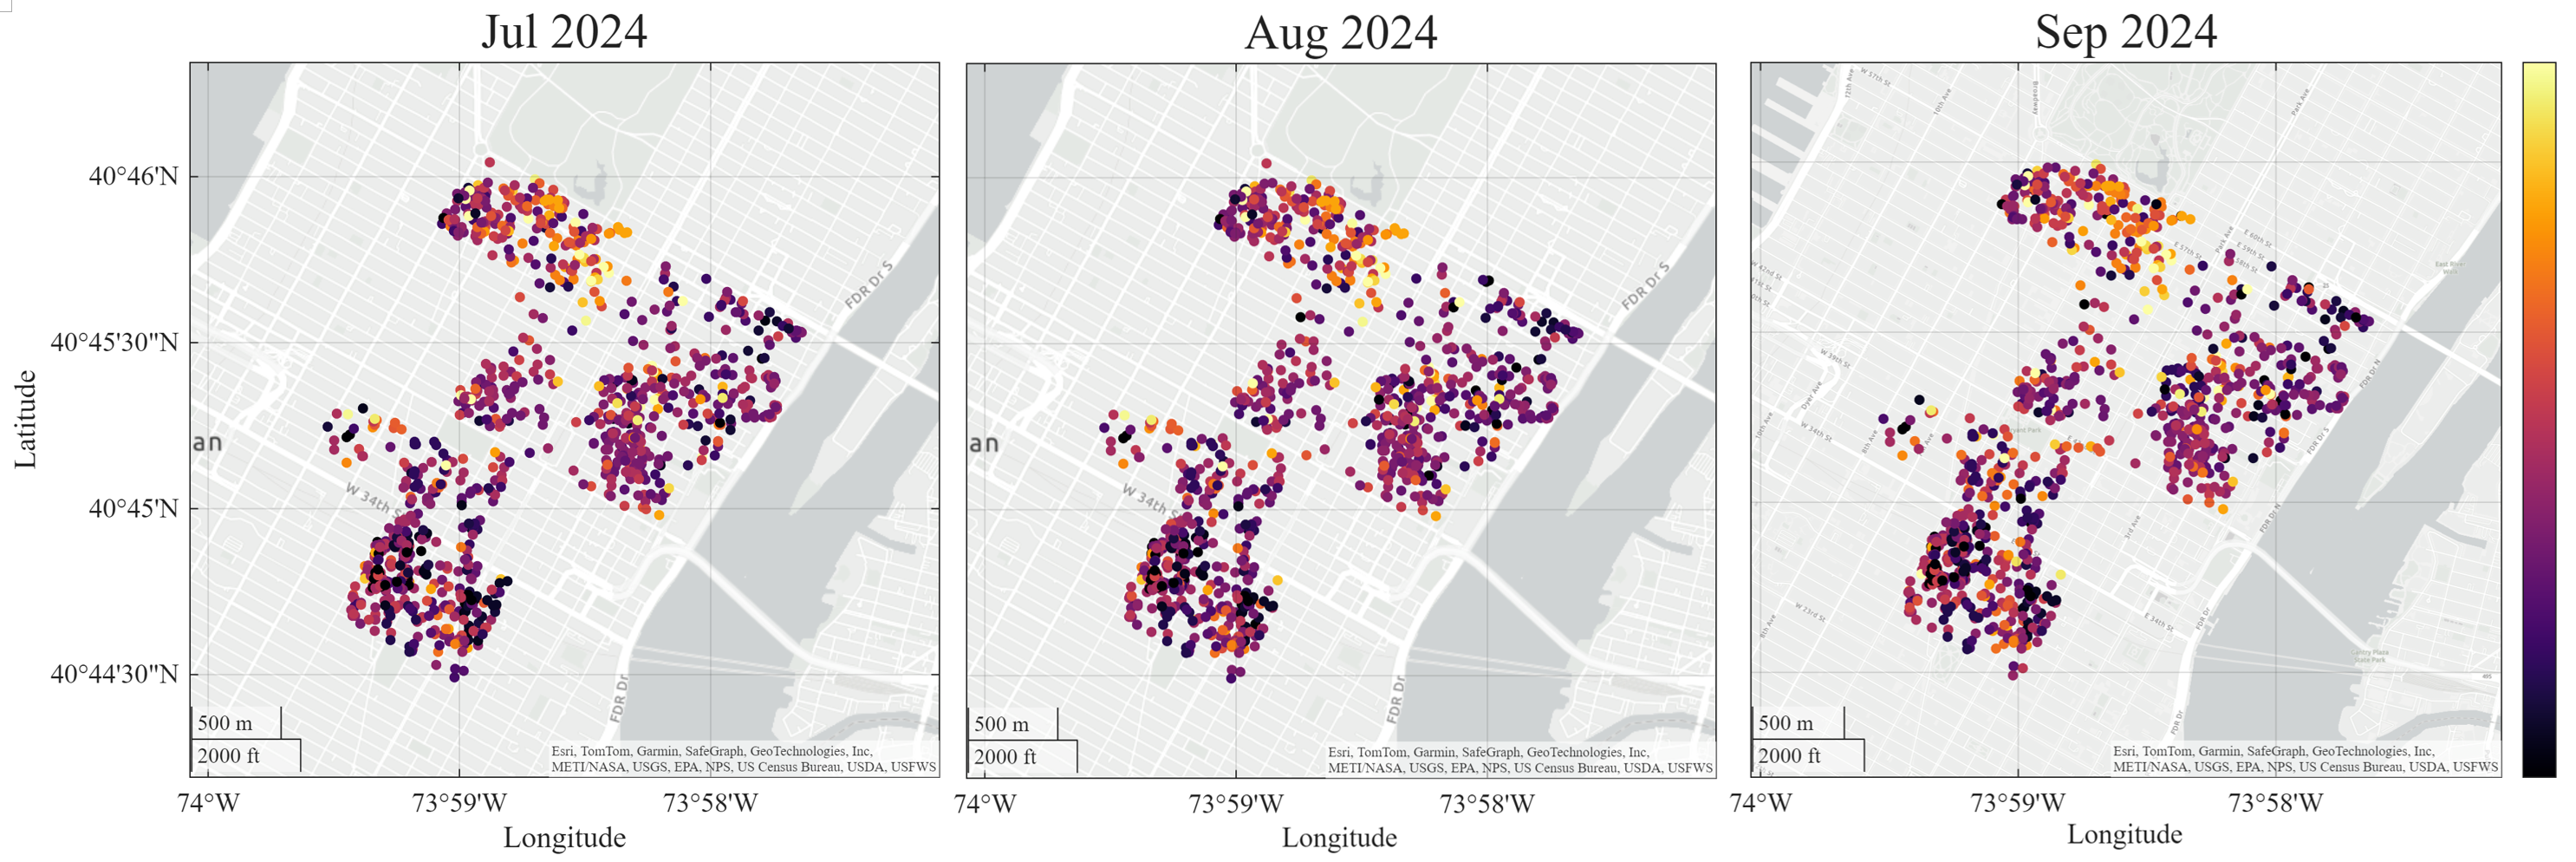
\includegraphics[width=\linewidth]{pic/GeoScatter.png}
    \caption{Geographical distribution of log rental prices in Midtown}
    \label{pic_geosc_MT}
\end{figure}

\begin{figure}[h]
    \centering
    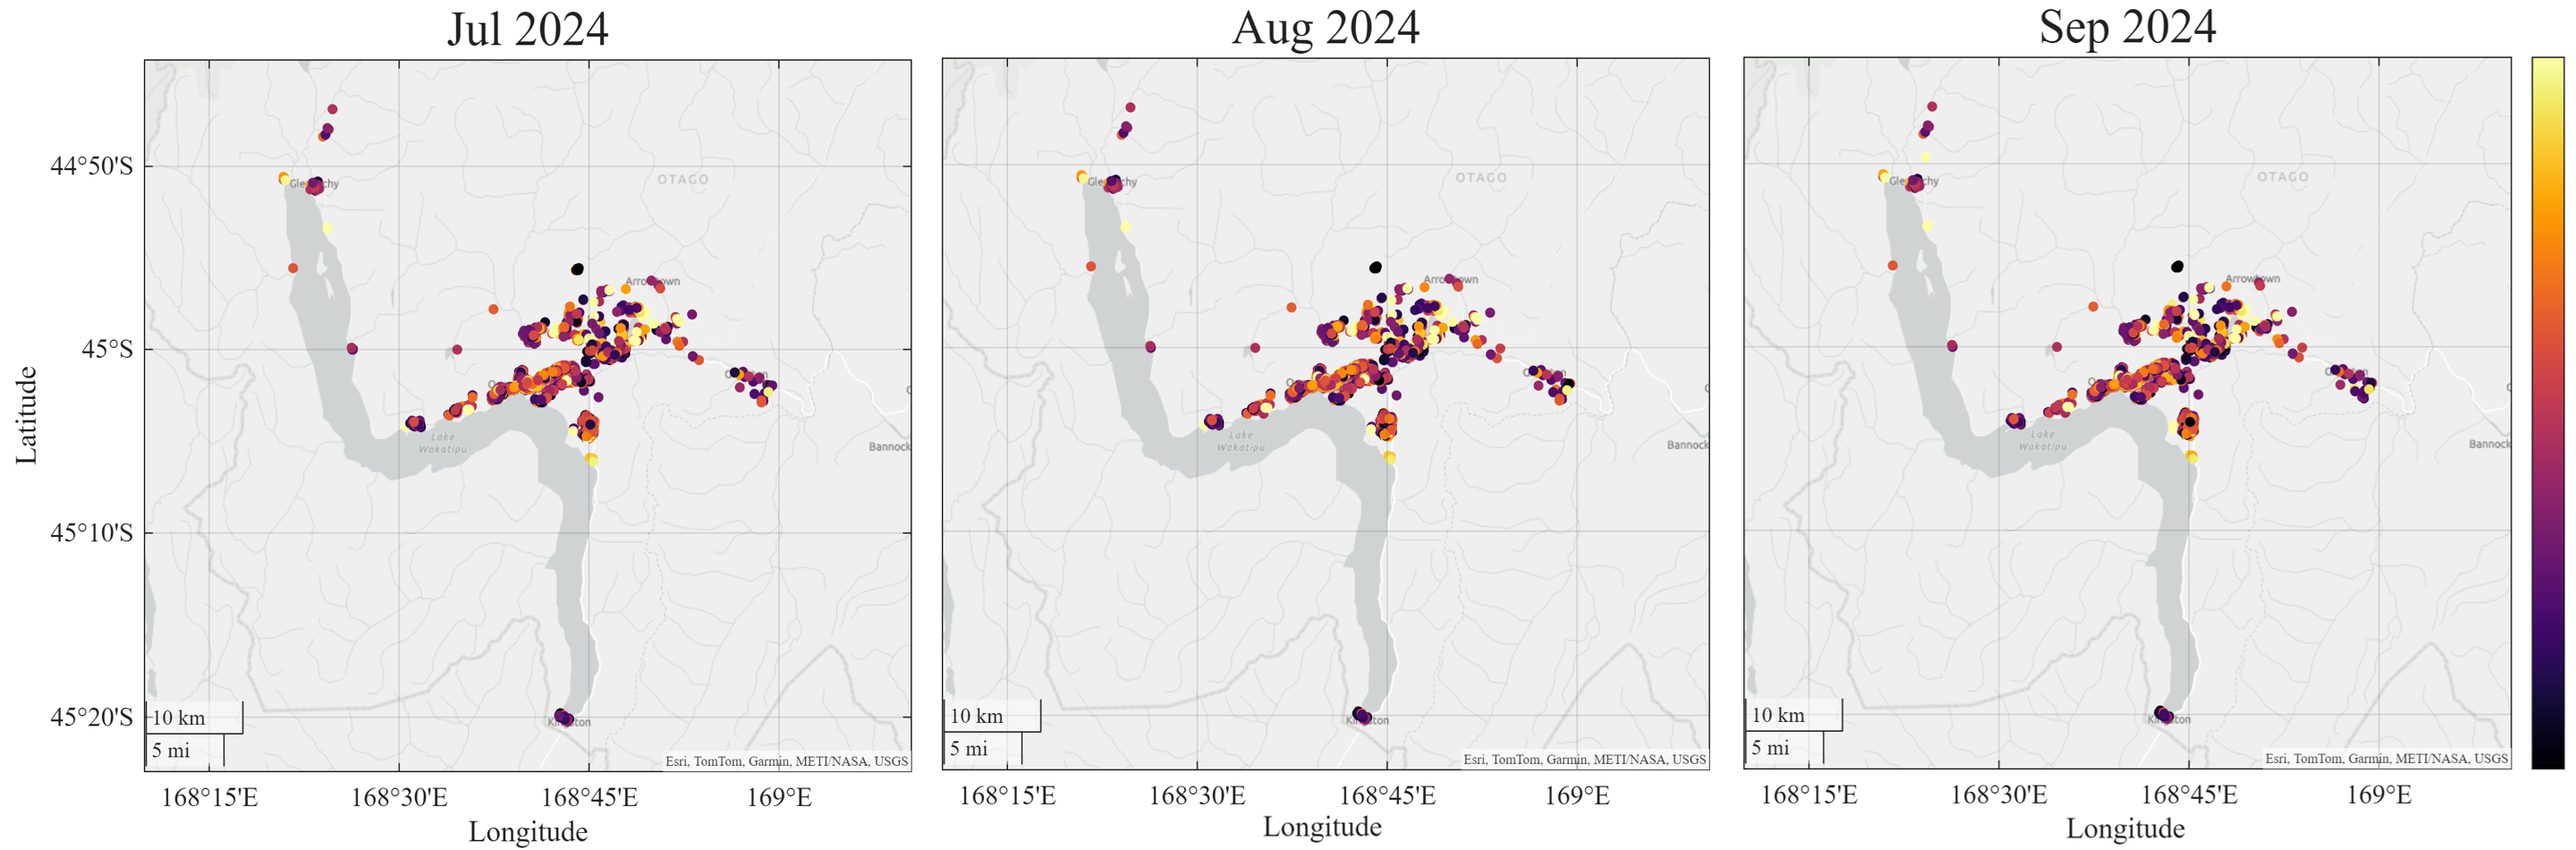
\includegraphics[width=\linewidth]{pic/GeoScatter2.png}
    \caption{Geographical distribution of log rental prices in Queenstown}
    \label{pic_geosc_QT}
\end{figure}

Based on the data described above, we estimate the TWFE unbalanced dynamic network panel model using the bias-corrected QMLE. For each local market, $W_t$ and $M_t$ are constructed as row-normalized binary distance-band matrices. Specifically, for a given distance threshold $d$, two listings are connected if their geographical distance is no larger than $d$. The contemporaneous matrix $W_t$ is constructed among listings observed in period $t$, with diagonal elements set to zero. The lagged matrix $M_t$ is constructed between listings observed in period $t$ and listings observed in period $t-1$, with links from a listing to itself in the previous period excluded. The resulting binary adjacency matrices are then row-normalized.
%Instead of using a common set of distance thresholds for all areas, we choose the thresholds adaptively because the New Zealand local markets and the New York City neighborhoods differ substantially in spatial scale. 
Instead of using a common set of distance thresholds for all areas, we choose the thresholds adaptively because the selected local markets differ substantially in spatial scale.
Specifically, the thresholds are selected based on the market-specific median nearest-neighbor distance and then rounded to one decimal place. This procedure yields thresholds of 0.4, 0.7, and 1.1 km for the three New Zealand local markets; 0.4, 0.6, and 1.1 km for Williamsburg; 0.1, 0.2, and 0.4 km for Midtown; and 0.2, 0.3, and 0.5 km for Hell's Kitchen. The main tables report the estimates under the largest distance threshold for each local market, while Supplementary Appendix E reports the estimates under all three thresholds.
%Instead of using a common set of distance thresholds for all areas, we choose the thresholds adaptively according to the spatial dispersion of listings in each local market. Specifically, the thresholds are selected based on the market-specific median nearest-neighbor distance and then rounded to one decimal place. This procedure yields thresholds of $0.4$, $0.7$, and $1.1$ km for the three New Zealand local markets; $0.4$, $0.6$, and $1.1$ km for Williamsburg; $0.1$, $0.2$, and $0.4$ km for Midtown; and $0.2$, $0.3$, and $0.5$ km for Hell's Kitchen. The main tables report the estimates under the largest distance threshold for each local market, while Supplementary Appendix E reports the estimates under all three thresholds.

Tables~\ref{Tab_Comv_TWFE} and~\ref{Tab_ComV_TWFE} compare the bias-corrected TWFE QMLE results across the selected local markets. The results are based on the same class of TWFE dynamic network model, but the distance thresholds are market-specific because of the adaptive construction described above. We obtain the following findings.

\begin{enumerate}[(1)]
\item The network autoregressive coefficient $\rho$ captures contemporaneous interaction effects among connected listings. It is positive and statistically significant in all six local markets. The estimates are larger in New York City, ranging from 0.4812 to 0.7690, than in New Zealand, where they range from 0.0960 to 0.1612. This difference is consistent with the higher listing density and stronger real-time competitive pressure in New York City. In contrast, listings in the New Zealand local markets are more geographically dispersed, which weakens contemporaneous spatial price transmission.

\item The lagged network autoregressive effect $\lambda$ captures the impact of neighboring prices in the previous period on current rental prices. This effect is significantly negative across all six local markets. Moreover, local markets with a larger contemporaneous network autoregressive coefficient $\rho$ generally exhibit a more negative estimate of $\lambda$. This pattern suggests an intertemporal dampening mechanism in network spillovers, whereby contemporaneous spatial interactions are partially attenuated by subsequent network effects.
%The lagged network autoregressive effect $\lambda$ captures the impact of neighboring prices in the previous period on current rental prices. This effect is significantly negative across all six local markets. The estimates are also more negative in New York City than in New Zealand, suggesting a stronger intertemporal dampening mechanism in denser urban rental markets.

\item The temporal lagged effect $\nu$ is positive and statistically significant in all local markets, indicating rental price persistence. The estimates range from 0.2082 to 0.3982 in New Zealand and from 0.3969 to 0.4638 in New York City.
\end{enumerate}


\begin{table}[H]
\centering
\caption{Bias-corrected TWFE QMLE estimates for New Zealand}\label{Tab_Comv_TWFE}
\begin{tabular}{llll}
\hline
\multicolumn{1}{c}{} & \multicolumn{1}{c}{Auckland} & \multicolumn{1}{c}{Queenstown} & \multicolumn{1}{c}{Wellington} \\
\hline
$\rho \quad (W_tY_t)$ & \phantom{-}0.1612(0.0053)*** & \phantom{-}0.0960(0.0055)*** & \phantom{-}0.1591(0.0333)*** \\
$\lambda \quad (M_tY_{t-1})$ & -0.1640(0.0053)*** & -0.0791(0.0052)*** & -0.0735(0.0301)** \\
$\nu \quad (Y_{t-1})$ & \phantom{-}0.3982(0.0031)*** & \phantom{-}0.3006(0.0028)*** & \phantom{-}0.2082(0.0049)*** \\
avail30d & -0.0006(0.0001)*** & -0.0005(0.0001)*** & -0.0003(0.0002)** \\
avgAvail30d1km & -0.0053(0.0004)*** & -0.0058(0.0004)*** & \phantom{-}0.0015(0.0016) \\
Listing effect & \phantom{-}0.2221(0.0059)*** & \phantom{-}0.2335(0.0064)*** & \phantom{-}0.1207(0.0274)*** \\
\cline{2-4}
$N$ & \multicolumn{1}{c}{5896} & \multicolumn{1}{c}{6095} & \multicolumn{1}{c}{1549} \\
$T$ & \multicolumn{1}{c}{30} & \multicolumn{1}{c}{30} & \multicolumn{1}{c}{30} \\
$n$ & \multicolumn{1}{c}{80716} & \multicolumn{1}{c}{95455} & \multicolumn{1}{c}{18723} \\
UP & \multicolumn{1}{c}{54.37\%} & \multicolumn{1}{c}{47.80\%} & \multicolumn{1}{c}{59.71\%} \\
\hline
\end{tabular}
\begin{flushleft}
\footnotesize
Notes: Estimates are presented with their standard errors in parentheses. Statistical significance is indicated by stars: *** for $p<0.01$, ** for $p<0.05$, and * for $p<0.1$.
\end{flushleft}
\end{table}

\begin{table}[H]
\centering
\caption{Bias-corrected TWFE QMLE estimates for New York City}\label{Tab_ComV_TWFE}
\begin{tabular}{llll}
\hline
\multicolumn{1}{c}{} & \multicolumn{1}{c}{Williamsburg} & \multicolumn{1}{c}{Midtown} & \multicolumn{1}{c}{Hell's Kitchen} \\
\hline
$\rho \quad (W_tY_t)$ & \phantom{-}0.7690(0.0310)*** & \phantom{-}0.4812(0.0238)*** & \phantom{-}0.5414(0.0267)*** \\
$\lambda \quad (M_tY_{t-1})$ & -0.5242(0.0397)*** & -0.2740(0.0319)*** & -0.4066(0.0328)*** \\
$\nu \quad (Y_{t-1})$ & \phantom{-}0.4638(0.0064)*** & \phantom{-}0.4597(0.0068)*** & \phantom{-}0.3969(0.0063)*** \\
avail30d & \phantom{-}0.0006(0.0002)*** & -0.0012(0.0003)*** & -0.0002(0.0003) \\
avgAvail30d1km & \phantom{-}0.0035(0.0031) & -0.0020(0.0034) & \phantom{-}0.0013(0.0093) \\
Listing effect & -0.0687(0.0438) & \phantom{-}0.2528(0.0420)*** & -0.0022(0.0380) \\
\cline{2-4}
$N$ & \multicolumn{1}{c}{1566} & \multicolumn{1}{c}{2390} & \multicolumn{1}{c}{1943} \\
$T$ & \multicolumn{1}{c}{17} & \multicolumn{1}{c}{17} & \multicolumn{1}{c}{17} \\
$n$ & \multicolumn{1}{c}{14567} & \multicolumn{1}{c}{23672} & \multicolumn{1}{c}{16862} \\
UP & \multicolumn{1}{c}{45.28\%} & \multicolumn{1}{c}{41.74\%} & \multicolumn{1}{c}{48.95\%} \\
\hline
\end{tabular}
\begin{flushleft}
\footnotesize
Notes: Estimates are presented with their standard errors in parentheses. Statistical significance is indicated by stars: *** for $p<0.01$, ** for $p<0.05$, and * for $p<0.1$.
\end{flushleft}
\end{table}
Furthermore, Tables E.2–E.7 in Supplementary Appendix E report detailed estimation results under different network weight matrix specifications for each area. Within each local market, the estimation results are generally similar across different distance-threshold specifications in terms of signs and statistical significance. A common pattern is that the absolute magnitudes of both the network autoregressive coefficient $\rho$ and the lagged network autoregressive effect $\lambda$ increase as the distance threshold d expands, while the remaining coefficients change only slightly. This pattern is consistent with the role of the distance threshold in defining the network exposure. Larger distance bands include a broader set of local competitors, which strengthens the measured contemporaneous network dependence and the subsequent lagged network adjustment. In contrast, the stability of the non-network coefficients suggests that the estimated effects of listing-level availability, nearby availability, temporal persistence, and listing entry are not driven by the particular distance-band choice.


\section{Conclusion}\label{section6}
In this paper, we study QMLE for genuinely unbalanced dynamic network panel data models as both $N$ and $T$ go to infinity. We first consider a baseline OWFE specification. For this specification, the QMLE is $\sqrt{NT}$-consistent for all parameters except for the listing effect $\hat{\gamma}$, which achieves $\sqrt{N}$-consistency. When $N$ grows proportionally to $T$, the QMLE has an asymptotic bias induced by the incidental parameters. The proposed bias-corrected estimator is asymptotically unbiased and normally distributed as long as $N/T^3 \to 0$. We also construct a consistent estimator of the asymptotic covariance matrix, making feasible inference available for the bias-corrected estimator.

We further extend the framework to a TWFE specification. Under this extension, the QMLE remains consistent, and the asymptotic bias contains an additional component generated by the estimation of time fixed effects. We derive the corresponding bias correction and show that the TWFE bias-corrected estimator is asymptotically unbiased and normally distributed when $N/T^3 \to 0$ and $T/N^3 \to 0$. A consistent estimator of the TWFE asymptotic covariance matrix is also provided.

Several extensions remain for future research. First, GMM estimation for this model is worth studying, because it can accommodate heteroskedastic errors and remains applicable when $T$ is finite. Second, building on the current TWFE extension, individual--time interactive fixed effects provide a natural direction for further development. Third, a more flexible mechanism for the listing effect is another promising extension.
%Several extensions remain for future research. First, GMM estimation for this model is worth studying, because it can accommodate heteroskedastic errors and remains applicable when $T$ is finite. Second, building on the current TWFE extension, individual--time interactive fixed effects provide a natural direction for further development. Third, a more flexible mechanism for the listing effect is another promising extension.

%In this paper, we consider the QMLE for a genuinely unbalanced dynamic network panel data model with individual fixed effects as both $N$ and $T$ go to infinity. 
%The QMLE is $\sqrt{NT}$-consistent for all parameters, except for the listing effect $\hat{\gamma}$, which achieves $\sqrt{N}$-consistency. While the QMLE is asymptotically biased when $N$ grows asymptotically faster than $T$, the bias-corrected estimator we propose is asymptotically unbiased and normally distributed as long as $\frac{N}{T^3}\to0$. 

%There are several extensions of this paper:
%(1) We are studying the GMM estimation for this model, as GMM allows for heteroskedasticity in the error terms, and is still consistent when $T$ is finite.
%(2) Building on this framework, temporal heterogeneous effects can also be incorporated into the model. In particular, extending the model to allow for TWFE and individual–time interactive fixed effects constitutes an important direction for future research.
%(3) A more complex mechanism for the listing effect is another promising extension.



\section*{Funding statement}
This work was supported by the National Natural Science Foundation of China (NSFC) under Grant Nos. 72473118, 72333001, and 71988101.

\section*{Competing interests}
The authors declare none.

\section*{Declaration of Generative AI Use}
During the preparation of this work the authors used ChatGPT in order to enhance the writing quality. After using this tool/service, the authors reviewed and edited the content as needed and take full responsibility for the content of the publication.

\section*{Data Availability Statement}
The data that support the findings of this study are available from Inside Airbnb at \url{https://insideairbnb.com}. These data were derived from publicly available monthly Airbnb listing snapshots.

\phantomsection\label{supplementary-material}
\section*{Supplementary Material}
The supplementary material includes the required lemmas and their proofs, the explicit expressions and properties of the QMLE score function and Hessian matrix, detailed proofs of the theorems, as well as tables and figures for the simulation and empirical results.

\section*{Acknowledgments}
We thank Professor Xiaoyu Meng, Chao Yang, Fei Jin, and Kai Yang for their valuable comments.

\bibliography{bibliography}
\end{document}
